% dãndòng 1,3 lines
% hai đoạn văn bản cách nhau 6pt và thụt dòng đầu của đoạn văn bản 1 cm.

\documentclass[13pt, a4paper]{report}
\usepackage[utf8]{vietnam}
\usepackage{unicode-math}
\usepackage{graphicx} % import graphics
\usepackage[a4paper]{geometry}
\geometry{top=2.5cm, bottom=3cm, left=3cm, right=2cm}
\graphicspath{ {./images/} }
\usepackage{titlesec}
\usepackage{listings}
\usepackage{float}
\usepackage{amsmath}
\usepackage{hyperref}
\usepackage{xcolor}
\usepackage{algorithm}
\usepackage{algpseudocode}
\usepackage{siunitx}
\usepackage{lmodern}
\usepackage{changepage}
\usepackage{tikz}
\usetikzlibrary{calc}

\linespread{1.3} 
\setlength{\parindent}{1cm} % Thụt dòng đầu của đoạn văn bản 1 cm
\setlength{\parskip}{6pt} % Hai đoạn văn bản cách nhau 6pt

%\renewcommand{\thesection}{\arabic{section}}

\hypersetup{
    colorlinks=true,
    linkcolor=blue,  
    urlcolor=cyan,
}

\newcommand{\dn}[1]{{\color{blue} [Dung: #1]}}
\newcommand{\an}[1]{{\color{red} [An: #1]}}

\newcommand{\myparagraph}[1]{\paragraph{#1}\mbox{}\\}
\setcounter{secnumdepth}{4}

\begin{document}
% Keywords command
\providecommand{\keywords}[1]
{
  % \small	
  \textbf{{Từ khóa: }} #1
}
\begin{titlepage}


\begin{tikzpicture}[overlay,remember picture]
  \draw [line width = 3pt]
   ($ (current page.north west) +(2.5cm, -2.0cm) $)
   rectangle
   ($ (current page.south east) + (-1.5cm,2.5cm) $);
  \draw [line width = 0.5pt]
  ($ (current page.north west) +(2.6cm, -2.1cm) $)
   rectangle
   ($ (current page.south east) + (-1.6cm,2.6cm) $);
\end{tikzpicture}
\begin{center}
{\bfseries\large ĐẠI HỌC QUỐC GIA HÀ NỘI \par}
{\bfseries\large TRƯỜNG ĐẠI HỌC CÔNG NGHỆ \par}
\vspace{10mm}
{
\includegraphics[width=0.25\textwidth]{images/logo/uet.png} \par}

\vspace{0.5cm}
{\bfseries\large KHOA CÔNG NGHỆ THÔNG TIN \par}
\vspace{0.5cm}

{\bfseries\huge KHOÁ LUẬN TỐT NGHIỆP \par}
\vspace{0.5cm}
{\mdseries\huge Tên công trình: Áp dụng quá trình ủ lượng tử
	\\ để giải bài toán xếp hậu \par}
\vspace{1cm}
\end{center}

{\large \textbf{Họ và tên sinh viên: Phùng Văn An} \par}
\vspace{0.3cm}


{\large \textbf{Lớp: K65-CC} \par}
\vspace{0.3cm}

{\large \textbf{Cán bộ hướng dẫn: TS. Nghiêm Nguyễn Việt Dũng} \par}
\vspace{0.3cm}

\vfill

\centering
{\bfseries\large Hà Nội, 2024 \par}
\end{titlepage}
\newpage
\thispagestyle{empty}
\centerline{\huge{\textbf{Lời cảm ơn}}}


Trước tiên, tôi xin gửi lời cảm ơn sâu sắc tới thầy Nghiêm Nguyễn Việt Dũng đã tận tình, đưa ra những lời khuyên và hướng dẫn tôi trong suốt thời gian làm khóa luận tốt nghiệp, cũng là người đã tạo điều kiện tốt nhất để tôi nghiên cứu về lĩnh vực lượng tử, một lĩnh vực thật sự khó. Lần đầu tôi được tiếp xúc với lĩnh vực lượng tử và nghiên cứu khoa học, kiến thức của tôi còn nhiều hạn chế nên không tránh khỏi những sai sót, tôi rất mong nhận được những ý kiến đóng góp quý giá của quý thầy cô để tôi có thể hoàn thiện hơn nữa khóa luận tốt nghiệp của tôi.

Tôi cũng xin cảm ơn các thầy cô trong khoa Công nghệ thông tin – Trường Đại
học Công Nghệ - Đại học quốc gia Hà Nội đã truyền đạt cho tôi những kiến thức
chuyên sâu về chuyên ngành trong suốt thời gian học tập để tôi có được nền tảng
kiến thức hỗ trợ rất lớn cho tôi trong quá trình làm khóa luận tốt nghiệp.

Sau cùng tôi xin tỏ lòng biết ơn đến cha mẹ, người thân và bạn bè đã luôn bên
cạnh để ủng hộ, động viên tôi trong cuộc sống để tôi có thể hoàn thành tốt luận
văn tốt nghiệp.

Xin chân thành cảm ơn! 


\newpage
\thispagestyle{empty}
\centerline{\huge{\textbf{Lời cam đoan}}}

"Tôi xin cam đoan các kết quả nghiên cứu, thực nghiệm được trình bày trong khóa luận này là do tôi thực hiện và được sự hướng dẫn của TS Nghiêm Nguyễn Việt Dũng, trước đây
chưa từng được sử dụng để làm khóa luận cho bất kỳ tổ chức giáo dục, hay trường
đại học nào khác."
\\
\\
\\
Chữ ký: ................................................

\newpage
\thispagestyle{empty}
\centerline{\huge{\textbf{Xác nhận của cán bộ hướng dẫn}}}

"Tôi xác nhận rằng khóa luận tốt nghiệp này đã đủ điều kiện để hội đồng đánh giá cho
chuyên ngành Công Nghệ Thông Tin tại Trường Đại học Công nghệ - Đại học Quốc Gia
Hà Nội."
\\
\\
\\
Chữ ký: ................................................

\newpage

\centerline{\textbf{Tóm tắt}}
\thispagestyle{empty}

Ủ lượng tử là một thuật toán tối ưu hóa lượng tử heuristic có thể được sử dụng để giải quyết các bài toán tối ưu hóa tổ hợp. Trong khóa luận này, chúng ta thảo luận về áp dụng quá trình ủ lượng tử để giải bài toán xếp hậu. Trong đó, chúng ta tận dụng lợi thế tính chất cơ bản của cơ học lượng tử. Nó bao gồm sự phát triển của một hệ thống hạt lượng tử (quantum bits). Chúng cùng nhau xác định dải năng lượng (energy landscape). Sau khi trải qua quá trình ủ đủ chậm, các hạt lượng tử có trạng thái tối ưu để tạo mức năng lượng thấp nhất cho toàn bộ hệ thống. Kết quả ở cuối quá trình ủ sẽ được đo nhiều lần. Nếu trong số những lần đo ta có được cấu hình với mức năng lượng thấp nhất thì cũng đồng nghĩa là tìm ra được lời giải tối ưu của bài toán. Ngoài ra, nếu không đạt được mức năng lượng thấp nhất, lời giải vẫn có ý nghĩa như là một lời giải tốt của bài toán.

Khóa luận này đã so sánh bài toán xếp hậu giữa các phương pháp cổ điển về mặt thời gian chạy. Cùng với đó cũng đã thử nghiệm công thức đề xuất của chúng ta, công thức cộng dồn, và so sánh ủ lượng tử và ủ mô phỏng trên bài toán xếp hậu. Kết quả thực nghiệm của ủ lượng tử dù còn chưa hiệu quả nhưng có hứa hẹn khi so với phương pháp mô phỏng luyện kim trên máy tính cổ điển. Trong tương lai, khi các máy lượng tử được cải tiến và nâng cấp, những bài toán NP-đầy đủ như bài toán xếp hậu với kích thước lớn có thể được giải thành công. 

Cấu trúc của khóa luận được trình bày như sau: Chương 1 giới thiệu bài toán xếp hậu, ủ lượng tử và lý do chọn đề tài. Trong Chương 2, chúng ta so sánh độ phức tạp thời gian của bài toán xếp hậu giữa các phương pháp cổ điển và giải thích các các công thức giải bằng ủ lượng tử. Chương 3, chúng ta sẽ thực nghiệm giữa các công thức và giữa ủ lượng tử và ủ mô phỏng, hiển thị kết quả thực nghiệm. Chương 4 kết luận từ kết quả thực nghiệm của phần trước đó và đề xuất hướng đi.
\newline
\newline
\keywords{bài toán xếp hậu, ủ lượng tử,  giải thuật mô phỏng luyện kim}

\onecolumn
\thispagestyle{empty}
\pagenumbering{gobble}
\tableofcontents
\thispagestyle{empty}
% \twocolumn
\clearpage




\thispagestyle{empty}
\listoffigures
\newpage
\thispagestyle{empty}
%\huge{\textbf{Danh sách từ viết tắt}}


\listoftables
\newpage

\thispagestyle{empty}


\newpage
\thispagestyle{empty}
{\huge{\textbf{Danh sách từ viết tắt}}}

\begin{figure}[H]
	\centering
	\begin{adjustwidth}{-1cm}{}
		\begin{center}
	\begin{tabular}{|l|l|l|}
		\hline
		SA & Simulated Annealing & Ủ mô phỏng \\
		\hline
		QA & Quantum Annealing & Ủ lượng tử \\
		\hline
		QUBO & Quadratic Unconstrained Binary Optimization & Bài toán tối ưu hóa nhị phân không ràng buộc bậc hai \\
		\hline
		BQM & Binary Quadratic Model & Mô hình bậc hai nhị phân \\
		\hline
		ID & Unique Number & Số duy nhất \\
		\hline
	\end{tabular}
\end{center}
\end{adjustwidth}
\end{figure}

\clearpage

\pagenumbering{arabic}
\chapter{Giới thiệu} 

Bài toán tối ưu hóa là bài toán cực đại hóa hoặc cực tiểu hóa một giá trị thực của hàm nhiều biến được gọi là hàm chi phí. Nếu bài toán là cực đại hóa hàm chi phí $f$ thì chỉ cần cực tiểu hóa $-f$ là đủ. Do đó, không mất tính tổng quát khi chỉ xem xét việc cực tiểu hóa.

Các bài toán tối ưu hóa được phân loại một cách tương đối thành hai loại, dễ và khó. Nói một cách đơn giản hơn, các bài toán dễ là những bài toán mà chúng ta có thuật toán để giải theo đa thức bước trong kích thước hệ thống (độ phức tạp đa thức). Ngược lại, đối với các bài toán khó, tất cả các thuật toán đã biết đều phải thực hiện rất nhiều bước theo cấp số nhân để đạt được lời giải chính xác (độ phức tạp theo cấp số nhân). Đối với những bài toán này, hầu như không thể tìm ra lời giải chính xác nếu kích thước bài toán vượt quá một giá trị vừa phải.

Trong khóa luận hiện tại, chúng ta sẽ thảo luận về các thuật toán tổng quát là ủ mô phỏng (Simulated Annealing) và ủ lượng tử (Quantum Annealing).

Trong SA, hàm chi phí cần giảm thiểu được xác định bằng năng lượng của hệ thống cơ học thống kê. Sau đó, hệ thống được cung cấp nhiệt độ, một tham số điều khiển được đưa vào một cách giả tạo, bằng cách giảm từ từ từ giá trị cao xuống 0, chúng ta hy vọng sẽ đưa hệ thống về trạng thái có giá trị năng lượng thấp nhất, đạt được lời giải của bài toán tối ưu hóa.

Trong các ứng dụng thực tế, SA rất phổ biến do khả năng áp dụng tổng quát, hiệu suất hợp lý và việc triển khai tương đối dễ dàng trong hầu hết các trường hợp. SA thường được sử dụng như một phương pháp để thu được nghiệm gần đúng trong thời gian tính toán hữu hạn vì nó cần một thời gian dài vô hạn để đạt được nghiệm chính xác bằng cách giữ hệ thống gần với trạng thái cân bằng nhiệt.

Trong SA, chúng ta sử dụng các dao động nhiệt (cổ điển) để cho phép hệ thống chuyển từ trạng thái này sang trạng thái khác vượt qua các rào cản năng lượng trung gian để tìm kiếm trạng thái năng lượng thấp nhất mong muốn.

Trong QA, chúng ta khéo léo kiểm soát cường độ của những dao động lượng tử này để hệ thống cuối cùng đạt đến trạng thái cơ bản, giống như SA, trong đó chúng ta giảm nhiệt độ từ từ và đường hầm lượng tử giữa các trạng thái cổ điển khác nhau thay thế bước nhảy nhiệt trong SA (Hình~\ref{fig:quantum_tunneling_and_hill_climbing}).

\begin{figure}[h]
	\centering
	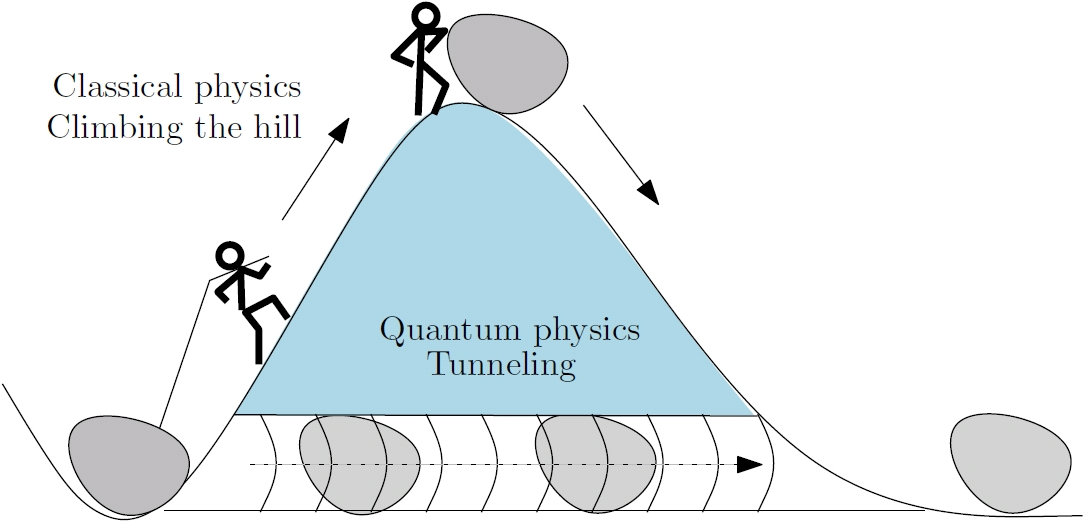
\includegraphics[width=0.7\textwidth]{images/quantum tunneling.png}
	\caption{Đường hầm lượng tử (trong QA) và bước nhảy nhiệt(leo đồi)(trong SA) \cite{Quantum tunneling}}
	\label{fig:quantum_tunneling_and_hill_climbing}
\end{figure}

Ý tưởng vật lý đằng sau quy trình như vậy là giữ cho hệ thống ở gần trạng thái cơ bản tức thời của hệ lượng tử, tương tự như trạng thái gần như cân bằng được giữ trong quá trình tiến hóa theo thời gian của SA. Tương tự như SA, về nguyên tắc, QA là một thuật toán tổng quát có thể áp dụng cho bất kỳ bài toán tối ưu hóa tổ hợp nào và được sử dụng như một phương pháp để đạt được lời giải gần đúng trong một khoảng thời gian hữu hạn nhất định.

%Người đọc có thể thắc mắc tại sao người ta lại phải phát minh ra một thuật toán tổng quát khác khi chúng ta đã có SA mạnh mẽ. Câu trả lời ngắn gọn là QA tốt hơn SA trong hầu hết các trường hợp, ít nhất là về mặt lý thuyết. Các kết quả phân tích và số học chỉ ra rằng thời gian tính toán cần thiết để đạt được độ chính xác nhất định của câu trả lời trong QA ngắn hơn so với SA. Ngoài ra, mức độ lỗi đối với QA nhỏ hơn SA nếu chúng ta chạy thuật toán trong một khoảng thời gian hữu hạn cố định.

%Một hạn chế của QA là việc triển khai thực tế đầy đủ phải dựa vào máy tính lượng tử vì chúng ta cần giải phương trình Schr¨odinger phụ thuộc thời gian ở quy mô rất lớn.


\section{Lý do chọn đề tài}
\subsection{Lý do chọn bài toán xếp hậu}


Bài toán xếp hậu là một bài toán kinh điển về bài toán NP-đầy đủ, được biết đến với tính chất thách thức của nó. Trong lĩnh vực tối ưu hóa và trí tuệ nhân tạo, nó có vai trò quan trọng trong nghiên cứu học thuật và ứng dụng thực tiễn như lý thuyết đồ thị, thiết kế mạch, điều khiển không lưu
, nén dữ liệu và lập lịch tác vụ máy tính \cite{A survey of known results and research areas for}. 
% Có thể nêu nhiều hơn ứng dụng hoặc chi tiết, cụ thể

\subsection{Lý do chọn ủ lượng tử}

Điện toán lượng tử (Quantum Computing) là một lĩnh vực nghiên cứu đang phát triển nhanh chóng, hứa hẹn một mô hình mới để giải quyết các bài toán tính toán đầy thách thức. Nó được giới thiệu lần đầu tiên vào đầu những năm 1980 bởi nhà vật lý Paul Benioff
\cite{The computer as a physical system}
và độc lập bởi Richard Feynman
\cite{Simulating physics with computers}.
Những đề xuất ban đầu này của điện toán lượng tử đề cập đến việc sử dụng các tính chất cơ bản của lượng tử như sự chồng chất (quantum superposition) và sự vướng víu (quantum entanglement) để thực hiện tính toán và mô phỏng tự nhiên. Trong những thập kỷ kể từ đó, những tiến bộ đáng kể của cả thuật toán và phần cứng đã mở rộng tiềm năng và phạm vi sử dụng của máy tính lượng tử. Các công trình chuyên đề của Deutsch 
\cite{Quantum computational networks}
và Grover 
\cite{A Fast Quantum Mechanical Algorithm for Database Search}
đã chỉ ra rằng các thuật toán lượng tử có thể mang lại sự tăng tốc tiệm cận (tăng tốc không đổi trong giới hạn kích thước hệ thống lớn) so với các lời giải cổ điển của chúng.
% đối  tác cổ điển??
Trong một số trường hợp, điều này thậm chí có thể dẫn đến các thuật toán nhanh hơn theo cấp số nhân, chẳng hạn như 
thuật toán biến đổi lượng tử Fourier
\cite{An approximate Fourier transform useful in quantum factoring}. 


Trong đề xuất của Deutsch \cite{Quantum computational networks}, điện toán lượng tử phổ quát theo mô hình đã trở thành "tiêu chuẩn" là mô hình mạch và mô hình cổng. Trong mô hình cổng, việc tính toán được thực hiện bằng cách áp dụng một chuỗi các cổng đơn nhất cho một tập hợp các hạt lượng tử (qubit), trạng thái của chúng có thể được đo khi kết thúc tính toán 
\cite{Quantum computational networks}
. Ngược lại, trong tính toán lượng tử đoạn nhiệt (Adiabatic Quantum Computing), người ta chuẩn bị trạng thái lượng tử nhiều hạt lượng tử ban đầu làm trạng thái cơ bản của Hamiltonian đơn giản, áp dụng tiến hóa thời gian đoạn nhiệt, thay đổi hệ thống thành Hamiltonian cuối cùng có trạng thái cơ bản, mã hóa lời giải mong muốn (tối ưu hóa) bài toán. 

Bất chấp những nỗ lực đáng kể về mặt lý thuyết     \cite{Adiabatic quantum computation} và thực nghiệm     \cite{Evidence for quantum annealing with more than one hundred qubits}, việc tăng tốc lượng tử trong tính toán lượng tử đoạn nhiệt vẫn chưa được chứng minh trong một thử nghiệm nào. Do đó, việc chứng minh lợi thế lượng tử bằng cách giải quyết các bài toán tối ưu hóa bằng các công cụ mô phỏng lượng tử là một bước quan trọng hướng tới sự phát triển của các bộ tối ưu 
% (general programmable quantum optimizers ?)
hóa lượng tử có thể lập trình tổng quát     \cite{A quantum annealin architecture with all-to-all connectivity from local interactions} \cite{Minor-embedding in adiabatic quantum computation: I. the parameter setting problem}.


\section{Giới thiệu về bài toán}
\subsection{Bài toán bao phủ chính xác (Exact Cover)}

Bài toán bao phủ chính xác có thể định nghĩa như sau: \cite{Ising formulations}

\textbf{Đầu vào: } Cho một tập $U = \{1, \dots, n \}$; và các tập con $V_i \subseteq U (i = 1, \dots, N)$ thoả mãn:

$$U = \bigcup_{i=1}^{} V_i$$


\textbf{Câu hỏi:} Liệu rằng có một tập con của tập các tập {$V_i$}, được gọi là R, sao cho các phần tử của R là các tập không giao nhau và hợp của các phần tử của R là U không?

Đây là một bài toán NP-đầy đủ.\\
Hàm Hamiltonian chúng ta sử dụng là: 
\[ H_A = A \sum_{\alpha=1}^{n} \left(1 - \sum_{i:\alpha \in V_i} x_i\right)^2\]

trong đó: $\alpha$ biểu thị các phần tử của U, $i$ biểu thị những tập con $V_i$. 

$H_A$ = 0 khi mỗi phần tử được đưa vào đúng một lần, hàm ý rằng các tập là không giao nhau. Sự tồn tại trạng thái năng lượng cơ bản H = 0 tương ứng với sự tồn tại nghiệm của bài toán bao phủ chính xác.

\subsection{Bài toán xếp hậu (N-Queens)}
Bài toán tám quân hậu lần đầu tiên được đề xuất bởi Max Bezzel trên một tạp chí cờ vua ở Berlin vào năm 1848 \cite{Proposal of eight queens problem}. Bài toán ban đầu là làm thế nào để đặt tám quân hậu lên bàn cờ sao cho không có quân hậu nào tấn công quân hậu khác. Bởi vì quân hậu được phép di chuyển bất kỳ khoảng trống nào theo chiều ngang, chiều dọc hoặc đường chéo, điều này có nghĩa là không quân hậu nào có thể ở cùng hàng, cột hoặc đường chéo với bất kỳ quân hậu nào khác.

Ví dụ, hình \ref{fig:8-queens-solution} đưa ra một lời giải cho bài toán tám quân hậu.

%\begin{figure}[h]
%	\centering
%	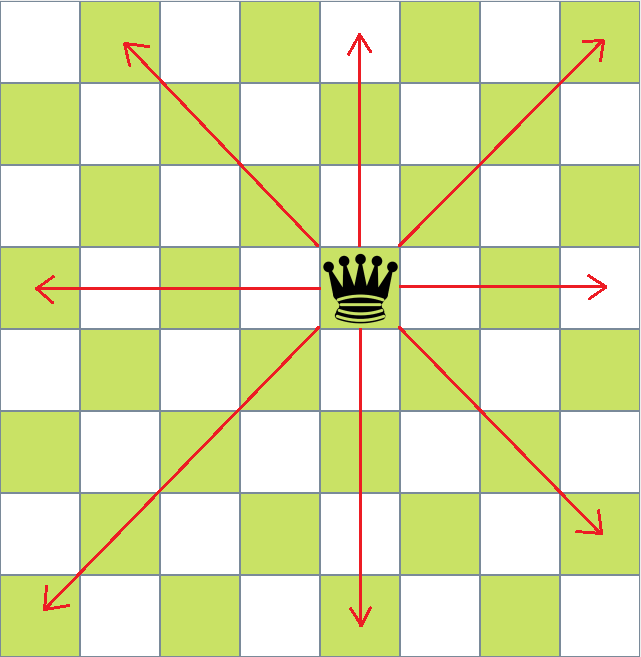
\includegraphics[width=0.5\textwidth]{images/direction-of-queen.png}
%	\caption{Các hướng đi của quân hậu}
%	\label{fig:direction-of-queen}
%	
%\end{figure}

\begin{figure}[h]
	\centering
	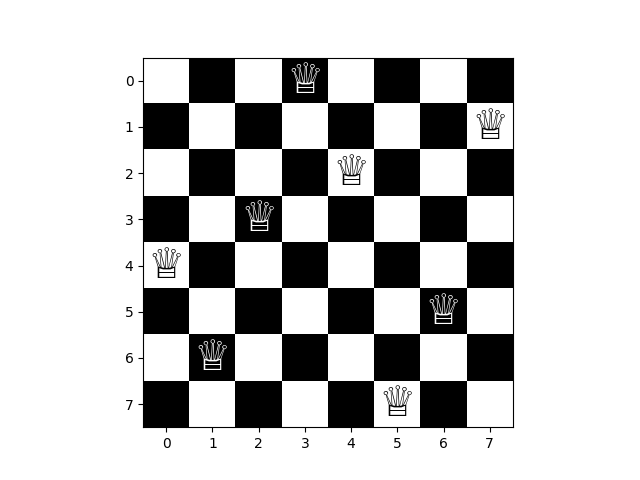
\includegraphics[width=0.7\textwidth]{images/8-queens-solution.png}
	\caption{Một lời giải cho bài toán tám quân hậu}
	\label{fig:8-queens-solution}
	
\end{figure}

Nếu số lượng quân hậu của bài toán được mở rộng, nó sẽ trở thành bài toán xếp hậu. 
Xếp hậu là một bài toán tối ưu hoá, dẫn xuất từ bài toán bao phủ chính xác. Cách tốt nhất để giải bài toán dạng này là áp dụng thuật toán vét cạn, quay lui và duyệt cây,\dots . Chúng ta tính toán tất cả các trường hợp cho tất cả các đầu vào có thể và xem xét giá trị hợp lệ . Tuy nhiên, cách tiếp cận này không phải lúc nào cũng có thể thực hiện được. Đôi khi, đầu vào số hậu không nhỏ.
May mắn thay, đó không phải là thuật toán duy nhất để giải bài toán dạng này. Có nhiều thuật toán có khả năng xác định điểm tối ưu mà không cần phải phân tích từng điểm của nó. Một trong số đó là ủ lượng tử.

\section{Ủ lượng tử}

\subsection{Nguyên lý hoạt động}
Ủ lượng tử là phiên bản lượng tử của quá trình ủ mô phỏng.
Ủ mô phỏng là một chiến lược xác suất được sử dụng để giải quyết các bài toán tối ưu hóa.

Không đi sâu vào chi tiết của thuật toán, chúng ta có thể giải thích ý tưởng đằng sau nó bằng cách nghĩ về một quả bóng lăn dọc theo đồ thị của hàm số, rơi vào các lỗ được xác định bởi cực tiểu. Mỗi khi một quả bóng rơi vào một cái lỗ, nó sẽ nhận được một lượng năng lượng nhất định, đủ để khiến nó nhảy qua một phần đồ thị khác, tìm kiếm những điểm cực tiểu sâu hơn. (Hình~\ref{fig:Quả bóng lăn dọc theo đồ thị hàm số})

\begin{figure}[h!]
    \centering
    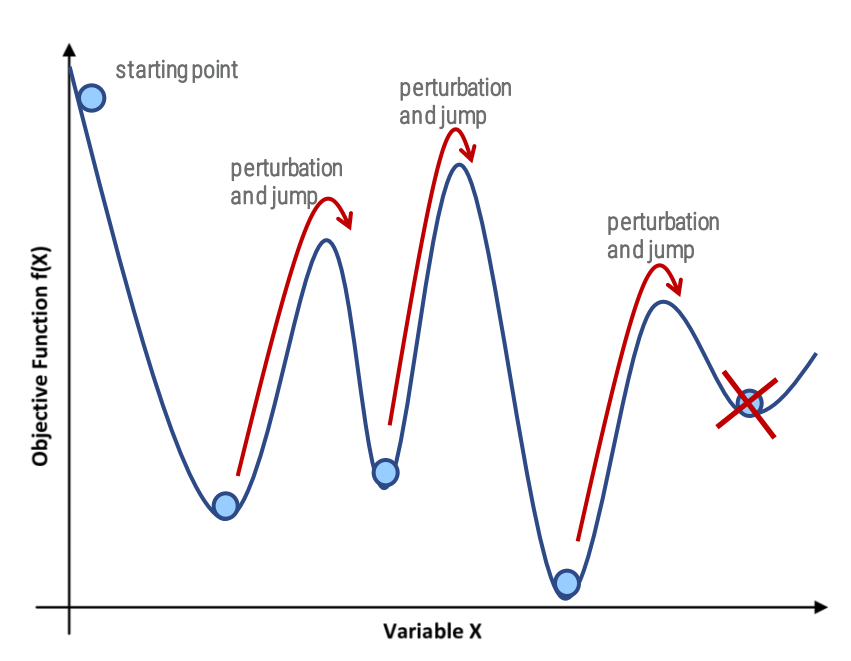
\includegraphics[width=0.7\textwidth]{images/SA.png}
     \caption{Đồ thị hàm số minh họa cho hàm mục tiêu trong ủ mô phỏng}
     \label{fig:Quả bóng lăn dọc theo đồ thị hàm số}
\end{figure}

 Về mặt trực quan, chúng ta có thể coi quá trình ủ lượng tử là một quá trình ủ mô phỏng trong đó quả bóng, một vật thể vĩ mô, được thay thế bằng một hạt cực nhỏ. 

Vậy quá trình ủ lượng tử diễn ra như thế nào? Cốt lõi của thuật toán nằm ở Định lý Đoạn nhiệt: Một hệ vật lý vẫn ở trạng thái riêng tức thời nếu một nhiễu loạn nhất định tác động lên nó đủ chậm và nếu có một khoảng cách giữa giá trị riêng và phần còn lại của phổ Hamilton.

Tối ưu hóa thông qua ủ lượng tử bắt đầu bằng việc chọn một hàm mục tiêu khác với hàm muốn tối ưu hóa. Sự lựa chọn thường rơi vào một hàm đơn giản. (Hình~\ref{fig:Đồ thị hàm số một hàm đơn giản})

\begin{figure}[h!]
    \centering
    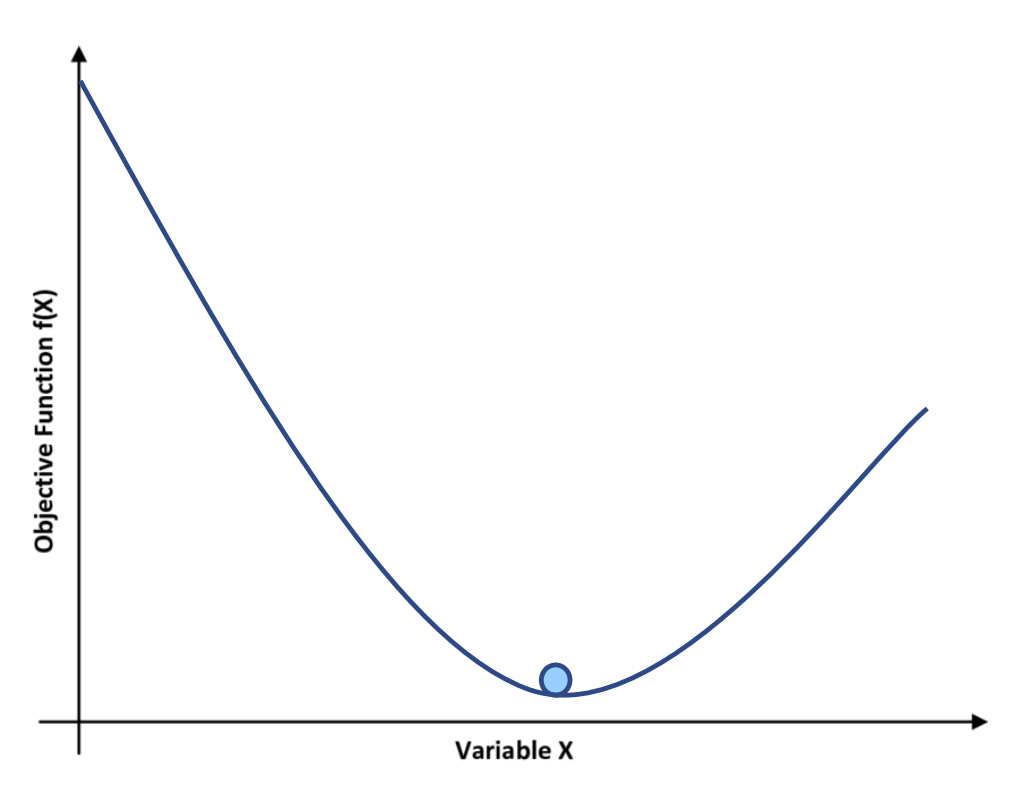
\includegraphics[width=0.7\textwidth]{images/simple_function.png}
    \caption{Hàm năng lượng khởi tạo là một hàm năng lượng đơn giản để đảm bảo trạng thái lượng tử ở mức năng lượng thấp nhất (ground state).}
    \label{fig:Đồ thị hàm số một hàm đơn giản}
\end{figure}

Quá trình ủ bao gồm việc sửa đổi từ từ hàm mục tiêu để thay đổi dần hình dạng của nó. Quá trình này kéo dài cho đến khi hàm mục tiêu ban đầu trở nên tương đương với hàm mục tiêu mà thực sự muốn tối ưu hóa. 
Nếu quá trình ủ diễn ra đủ chậm thì Định lý Đoạn nhiệt đảm bảo với chúng ta rằng trong tất cả các giai đoạn biến đổi của hàm mục tiêu, điểm cực tiểu toàn cục đã thích ứng với hình dạng của hàm. (Hình~\ref{fig:Biến đổi hàm mục tiêu})

\begin{figure}[h!]
    \centering
    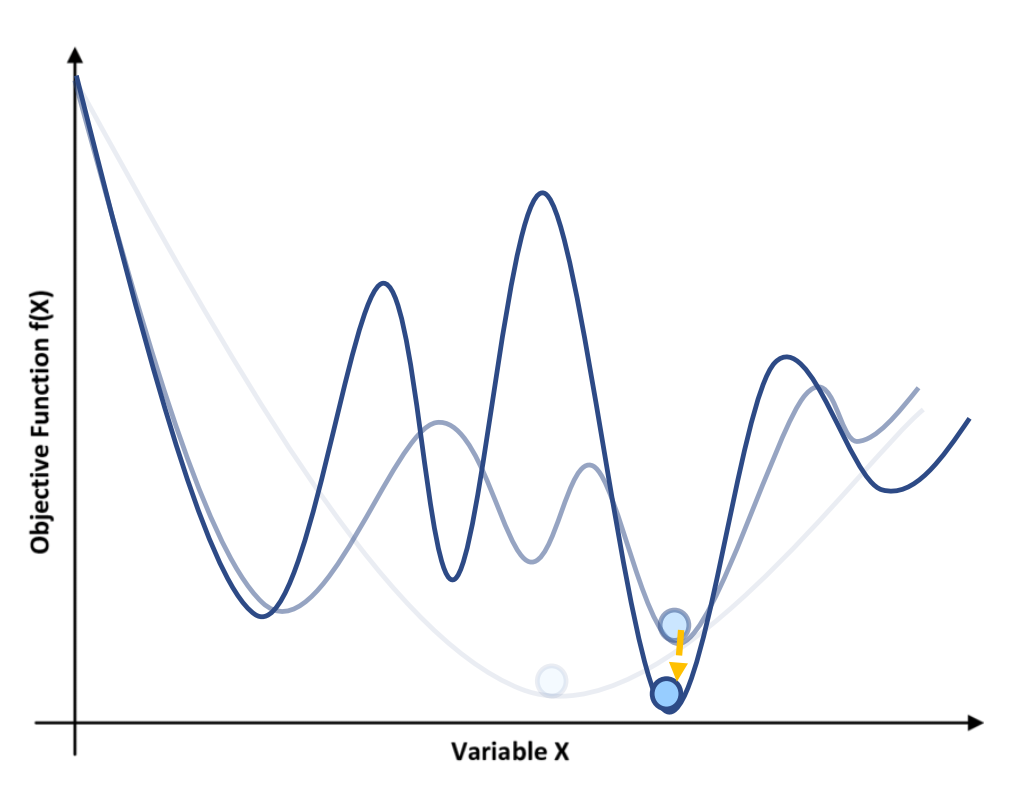
\includegraphics[width=0.7\textwidth]{images/QA.png}
    \caption{Quá trình ủ lượng tử từ từ diễn ra đủ chậm thì trạng thái lượng tử vẫn giữ ở mức năng lượng thấp nhất}
    \label{fig:Biến đổi hàm mục tiêu}
\end{figure}

Để hiểu cách tương tác với máy ủ lượng tử, chúng ta cần các khái niệm sau:

\begin{itemize}
  \item Hàm mục tiêu
  \item Bài toán tối ưu hóa nhị phân không ràng buộc bậc hai (QUBO)
  \item Đồ thị và nhúng
  
\end{itemize}

\subsection{Hàm mục tiêu và ràng buộc}


Để biểu diễn một bài toán giải quyết nó thông qua quá trình ủ lượng tử, trước hết chúng ta cần một hàm mục tiêu. Hàm mục tiêu là một biểu thức toán học của năng lượng của một hệ thống. Nói một cách đơn giản, nó đại diện cho hàm có giá trị tối thiểu mà bạn muốn tìm và năng lượng ở đây là hàm của các biến nhị phân đại diện cho hạt lượng tử của nó. (Hình~\ref{fig: Đồ thị năng lượng hàm mục tiêu})

\begin{figure}[H]
    \centering
    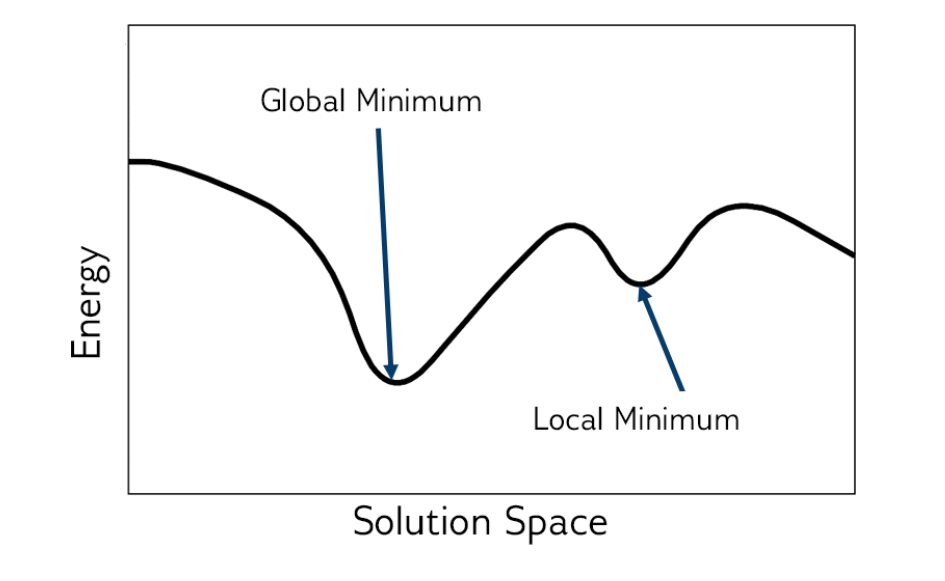
\includegraphics[width=0.7\textwidth]{images/objective_function.png}
    \caption{Nếu quá trình ủ diễn ra nhanh hoặc do nhiễu của thiết bị thì xác suất chính của trạng thái lượng tử rơi vào cực trị địa phương, làm bài toán không tìm được lời giải tối ưu.}
    \label{fig: Đồ thị năng lượng hàm mục tiêu}
\end{figure}

Trong hầu hết bài toán, năng lượng càng thấp thì lời giải càng tốt. Đôi khi bất kỳ trạng thái năng lượng tối thiểu cục bộ nào cũng là một lời giải có thể chấp nhận được cho bài toán ban đầu; đối với các bài toán khác chỉ có lời giải tối ưu mới được chấp nhận.

\subsection{Bài toán tối ưu hóa nhị phân không ràng buộc bậc hai (QUBO)}
Bài toán tối ưu hóa nhị phân không ràng buộc bậc hai là bài toán nổi tiếng trong lĩnh vực tối ưu hóa tổ hợp.
Bài toán QUBO được xác định bằng ma trận đường chéo Q, là một ma trận tam giác trên N x N  có trọng số thực và x, một vectơ của các biến nhị phân.\\
Hàm mục tiêu được biểu diễn dưới dạng bài toán QUBO như sau:
\[\text{E}_{qubo}(a_i, b_{i,j}; q_i) = \sum_{i} a_i q_i + \sum_{i<j} b_{i,j} q_i q_j.
\]
Trong đó các số hạng đường chéo của ma trận Q đóng vai trò là hệ số tuyến tính, còn các phần tử khác 0 là hệ số bậc hai
\[\min_{{x} \in {\{0,1\}^n}} {x}^{T} {Q}{x}.
\]

Hàm phạt là một đại lượng bổ sung cho bài toán tối ưu hóa ban đầu, đại lượng này phải được tối ưu hóa để toàn bộ bài toán được tối ưu hóa.

\subsection{Đồ thị và nhúng}
Về mặt toán học, đồ thị vô hướng được định nghĩa là một tập hợp các đỉnh
(V) và tập các cạnh (E)
Mỗi đỉnh và mỗi cạnh có thể được đánh trọng số.
Bằng cách này, có thể thiết lập sự tương ứng một-một giữa đồ thị có trọng số và hàm QUBO.

Cốt lõi của máy ủ lượng tử được biểu thị bằng đồ thị: trong hình~\ref{fig: Pegasus_qubits}, chúng ta có thể quan sát ô đơn vị của cấu trúc liên kết Chimera, đó là cấu trúc liên kết của một trong các mô hình D-Wave.
Điều này có nghĩa là để giải bài toán QUBO, cần phải ánh xạ bài toán lên đồ thị của máy ủ lượng tử đã chọn. Thủ tục này gọi là nhúng.

\begin{figure}[H]
    \centering
    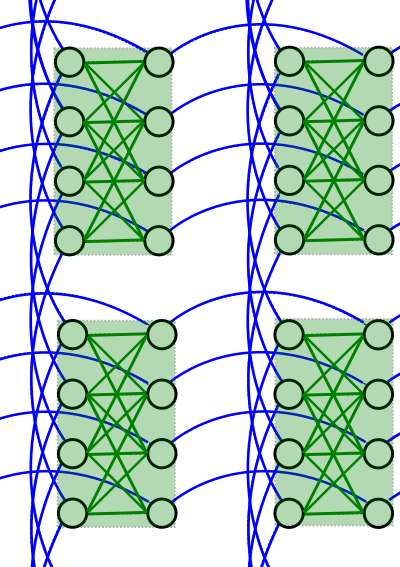
\includegraphics[width=0.5\textwidth]{images/Chimera_2x2_unit_cells.png}
    \caption{Hai ô đơn vị của biểu đồ Chimera. Hạt lượng tử được sắp xếp thành 4 ô đơn vị (hình vuông màu xanh lục mờ) được kết nối với nhau bằng bộ ghép bên ngoài (đường màu xanh lam) \cite{Topologies}}
    \label{fig: Pegasus_qubits}
\end{figure}



% Các biến thể của bài toán


\chapter{Phương pháp}
\section{Phương pháp giải cổ điển}

\subsection{Thuật toán quay lui (backtracking) với bài toán xếp hậu}
Các bước thực hiện thuật toán quay lui với bài toán xếp hậu như sau:
\begin{enumerate}
    \item Khởi tạo một bàn cờ rỗng với kích thước NxN, đánh dấu tất cả các ô trên bàn cờ là chưa đặt quân hậu.
    \item Bắt đầu từ hàng đầu tiên, đặt quân hậu vào từng ô trên hàng đó. Với mỗi ô, kiểm tra xem nó có bị tấn công bởi quân hậu nào đã đặt trên bàn cờ hay không. Nếu không, đánh dấu ô đó là đã đặt quân hậu và tiếp tục đệ quy để đặt quân hậu trên hàng tiếp theo.
    \item Nếu không tìm được ô trống nào trên hàng đó để đặt quân hậu, quay trở lại hàng trước đó và thử đặt quân hậu vào ô tiếp theo trên hàng đó.
    \item Nếu đã đặt được N quân hậu trên bàn cờ, lưu trữ kết quả và thoát khỏi đệ quy.
    \item Nếu đã kiểm tra tất cả các ô trên bàn cờ nhưng không tìm được cách đặt quân hậu hợp lệ, quay trở lại và thử cách đặt quân hậu khác.
    % \item Khi đã thử tất cả các ô trên bàn cờ và lưu giữ được tất cả các lời giải, kết thúc thuật toán và trả về các lời giải đã tìm được.
\end{enumerate}

\textbf{Triển khai thuật toán:}

\begin{algorithm}[H]

\caption{Thuật toán quay lui cho bài toán xếp hậu}
\begin{algorithmic}[1]
\State $vertical = [0] * n$
\State $main\_diag =  [0] * (2 * n - 1)$
\State $anti\_diag = [0] * (2 * n - 1)$

\State
\Function{solve\_n\_queens}{n}
    \State Create an empty board of size $n \times n$
    \If{\Call{solve\_n\_queens\_util}{board, 0, n} is False}
        \State \textbf{print} "Solution does not exist"
    \EndIf
    \State \Return board
\EndFunction
\State
\Function{solve\_n\_queens\_util}{board, row, n}
    \If{row is equal to n}
        \State \Return True
    \EndIf
    \For{$col \gets 0$ \textbf{to} $n-1$}
        \If{\Call{is\_safe}{row, col, n}}
            \State Place a queen at board[row][col]
            \If{\Call{solve\_n\_queens\_util}{board, row+1, n} is True}
                \State \Return True
            \EndIf
            \State Remove the queen from board[row][col]
        \EndIf
    \EndFor
    \State \Return False
\EndFunction
\State
\Function{is\_safe}{row, col, n}
    	
        \If{vertical[col] is 1}
            \State \Return False
        \EndIf
    
  		\State $idx\_main \gets (row - col + n - 1)$
        \If{main\_diag[idx\_main] is 1}
            \State \Return False
        \EndIf

   		\State $idx\_anti \gets (row + col)$
        \If{anti\_diag[idx\_anti] is 1}
            \State \Return False
        \EndIf
    
    \State \Return True
\EndFunction
\end{algorithmic}
\end{algorithm}

Trong đó, hàm \textsc{is\_safe} kiểm tra xem một ô trên bàn cờ có thể đặt quân hậu hay không, và \textsc{solve\_n\_queens\_util} là hàm đệ quy sử dụng kỹ thuật quay lui để thử tất cả các cách đặt quân hậu trên bàn cờ. Hàm \textsc{solve\_n\_queens} tạo một bàn cờ rỗng và trả về lời giải hợp lệ.

Độ phức tạp về thời gian của thuật toán có thể được biểu thị bằng O(N!) vì trong trường hợp xấu nhất, yêu cầu phải thử tất cả các ô, tuy nhiên mỗi lần sẽ số hàng , cột giảm đi một.

\subsection{Thuật toán quy hoạch động với bài toán xếp hậu}
Thuật toán quy hoạch động cho bài toán xếp hậu được xây dựng bởi Rivin, I. và Zabih, R.\cite{dynamic programming solution} với độ phức tạp $O( f(N)*(8^N))$, với $f(N) = N^2g(N)$ là đa thức bậc thấp, $g(N)$ xuất phát từ độ phức tạp của số học số nguyên, cho bài toán xếp hậu đã chứng minh ưu việt hơn đối với cách tiếp cận quay lui đã đề cập bên trên.

Thuật toán được mô tả như sau:

Với một tập hợp các bộ dữ liệu $\langle S, i\rangle$, trong đó $S$ là tập hợp các đường (đã đặt hậu) và $i$ là một số nguyên, thể hiện một lớp tương đương của i ứng viên khả thi có tập hợp các đường đã đặt hậu là S, ta có các bước thực hiện:
\begin{enumerate}
	\item[1.] [Khởi tạo] Đặt QUEUE thành $\{\langle\emptyset, 1\rangle \}$.
	\item[2.] [Chọn ô vuông] Chọn một ô vuông chưa kiểm tra. Gọi $T$ là tập hợp bốn đường chứa ô vuông này
	\item[3.] [Vòng lặp] Với mọi tập $\langle S, i\rangle \in \text{QUEUE}$ sao cho $S \cap T = \emptyset$ thì:
	\begin{enumerate}
		\item[3.1] [Nén] Nếu $\langle S \cup T, j\rangle \in \text{QUEUE}$ đối với $j$ bất kỳ, thay $j$ bằng $i + j$.
		\item[3.2] [Tạo] Nếu không, hãy thêm $\langle S \cup T, i \rangle$ vào $\text{QUEUE}$.
	\end{enumerate}
	\item[4.] [Kết thúc] Nếu vẫn còn một ô vuông chưa được kiểm tra, hãy chuyển sang bước 2. Nếu không, hãy kết thúc.
\end{enumerate}



\section{Phương pháp giải bằng ủ lượng tử}

\subsection{Công thức bình phương cho bài toán xếp hậu}


Đầu tiên, chúng ta trình bày công thức QUBO được đề xuất bởi D-wave \cite{N Queens Dwave} sử dụng O($N^2$) biến. 
Nhưng làm cách nào để diễn đạt bài toán này dưới dạng mô hình bậc hai nhị phân(BQM)?

Để ánh xạ bài toán dưới dạng mô hình bậc hai nhị phân, chúng ta thực hiện các bước:\cite{Problem Formulation Guide} 


\textbf{Bước 1: Viết ra mục tiêu và các ràng buộc}

\textbf{Mục tiêu}: Không


\textbf{Ràng buộc}:
\begin{enumerate}
	\item Có chính xác một quân hậu trên mỗi hàng.
	\item Có chính xác một quân hậu trên mỗi cột.
	\item Có nhiều nhất một quân hậu nằm trên mỗi đường chéo chính (từ trên cùng bên trái đến dưới cùng bên phải).
	\item Có nhiều nhất một quân hậu nằm trên mỗi đường chéo phụ (từ dưới cùng bên trái đến trên cùng bên phải).
	
\end{enumerate}

\textbf{Bước 2: Chuyển đổi mục tiêu và các ràng buộc thành biểu thức toán nhị phân}

\textbf{Biến nhị phân:} Đầu tiên, chúng ta cần xác định các biến nhị phân của mình. Câu trả lời mà chúng ta đang tìm kiếm là chúng ta nên chọn ô nào. Với mỗi ô, chúng ta có thể hỏi “Chúng ta có chọn ô này để đặt hậu không?”. 

\begin{table}[H]
	\centering
	\begin{tabular}{ c c c }
		\hline
		& \textbf{Chọn ô [i,j]} & \textbf{Không chọn ô [i,j]} \\
		\hline
		\textbf{\textbf{QUBO}}     & $x_{ij} = 1$& $x_{ij} =0 $  \\
		
		\hline
	\end{tabular}
	
	
\end{table}

Khi đã xác định được các biến nhị phân, chúng ta có thể chuyển đổi mục tiêu và ràng buộc thành các biểu thức toán học.


\textbf{Mục tiêu}: Không

\textbf{Ràng buộc}:

Xét tập $Q = \{ Q_{ij} \text{ với } i, j = 1,2, \dots , n\}$, mỗi $Q_{ij}$ là một biến nhị phân với các giá trị \{0, 1\} tương ứng ô \{i, j\} không đặt và đặt quân hậu.
\begin{enumerate}
	
	\item Có chính xác một quân hậu trên mỗi hàng. 
	
	Xét tập $R = \{R_1, R_2, \dots R_n\}$, trong đó $R_u$ là tập quân hậu $Q_{ij}$ sao cho $i = u; j = 1,2, \dots , n$, ta có:
	\[
	\sum{R_u} = 1 \\ 
	\]
	
	
	\item Có chính xác một quân hậu trên mỗi cột.
	
	Xét tập $C = \{C_1, C_2, \dots C_n\}$, trong đó $C_u$ là tập quân hậu $Q_{ij}$ sao cho $i = 1,2, \dots , n; j = u$, ta có:
	\[
	\sum{C_u} = 1 \\ 
	\]
	
	\item Có nhiều nhất một quân hậu nằm trên mỗi đường chéo chính (từ trên cùng bên trái đến dưới cùng bên phải).
	
	Xét tập $D = \{D_{1-n}, D_{2-n}, \dots D_{n-1}\}$, trong đó $D_u$ là tập quân hậu $Q_{i,j}$ sao cho $i-j =u$, ta có:
	
	\[
		\sum{D_u}  \leq 1
	\]
	
	\item Có nhiều nhất một quân hậu nằm trên mỗi đường chéo phụ (từ dưới cùng bên trái đến trên cùng bên phải).
	
	Xét tập $A = \{A_2, A_3, \dots A_{2n}\}$, trong đó $A_u$ là tập quân hậu $Q_{i,j}$ sao cho $i+j =u$, ta có:
	
	\[
		\sum{A_u}  \leq 1 
	\]
	
	
	
\end{enumerate}

\textbf{Bước 3: Chuyển đổi biểu thức toán học thành mô hình bậc hai nhị phân}


Vì có chính xác một quân hậu trên mỗi hàng và cột, nên chúng ta sử dụng phiên bản tổng quát của thuật toán bao phủ chính xác \cite{Ising formulations} để xử lý các ràng buộc hàng và cột. 

Ràng buộc 1: Có chính xác một quân hậu trên mỗi hàng. (Hình \ref{fig:row-square-constraint})

\[
H_1 = \sum_{u}^{}{(1-\sum{}^{}{R_u})^2}
\]

\begin{figure}[H]
	\centering
	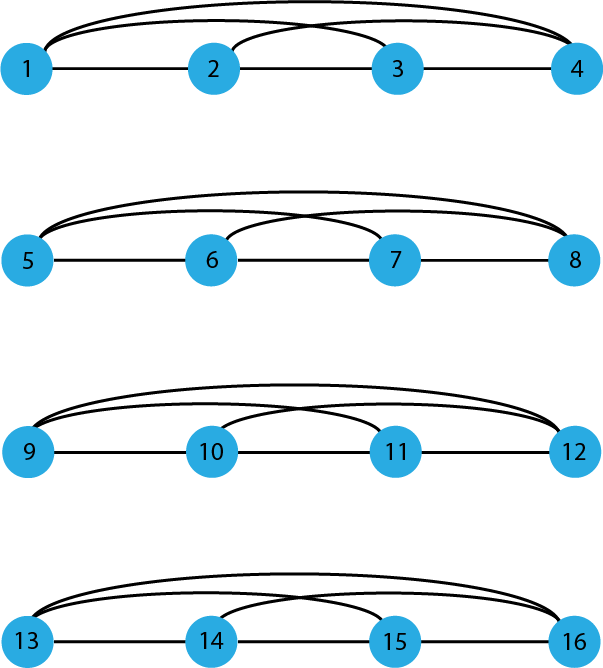
\includegraphics[width=0.5\textwidth]{images/row-square-constraint.png}
	\caption{Minh họa liên kết các ô trong ràng buộc hàng với N = 4 trong công thức bình phương}
	\label{fig:row-square-constraint}
\end{figure}


Ràng buộc 2: Có chính xác một quân hậu trên mỗi cột. (Hình \ref{fig:col-square-constraint})

\[
H_2 = \sum_{u}^{}{(1-\sum{}^{}{C_u})^2}
\]
\begin{figure}[H]
	\centering
	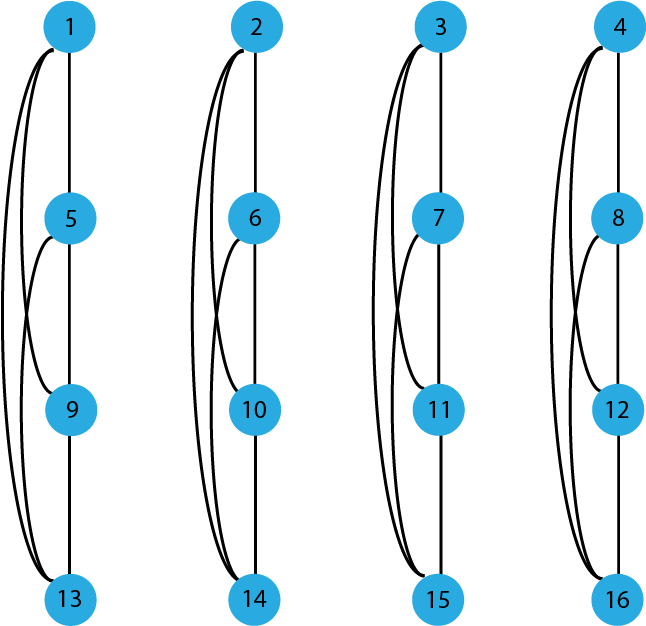
\includegraphics[width=0.5\textwidth]{images/col-square-constraint.png}
	\caption{Minh họa liên kết các ô trong ràng buộc cột với N = 4 trong công thức bình phương}
	\label{fig:col-square-constraint}
\end{figure}


Ràng buộc 3: Có nhiều nhất một quân hậu nằm trên mỗi đường chéo chính (từ trên cùng bên trái đến dưới cùng bên phải). (Hình \ref{fig:main-diag-square-constraint})

Xét $D_{ui}, D_{uj}$ tương ứng là phần tử thứ i, j của tập $D_u$, ta có:

\[
H_3 = \sum_{u}^{}{( \sum_{i<j}^{}{D_{ui}D_{uj}})}
\]

\begin{figure}[H]
	\centering
	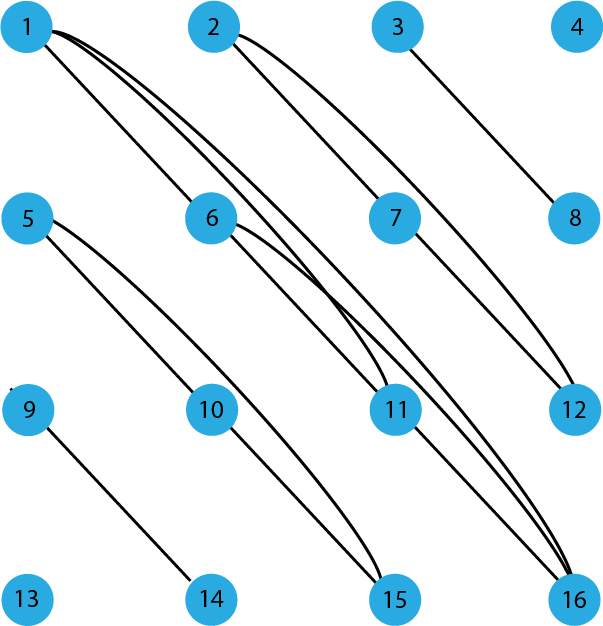
\includegraphics[width=0.5\textwidth]{images/main-diag-square-constraint.png}
	\caption{Minh họa liên kết các ô trong ràng buộc đường chéo chính với N = 4 trong công thức bình phương}
	\label{fig:main-diag-square-constraint}
\end{figure}


Ràng buộc 4: Có nhiều nhất một quân hậu nằm trên mỗi đường chéo phụ (từ dưới cùng bên trái đến trên cùng bên phải). (Hình \ref{fig:anti-diag-square-constraint})

Xét $A_{ui}, A_{uj}$ tương ứng là phần tử thứ i, j của tập $A_u$, ta có:

\[
H_4 = \sum_{u}^{}{( \sum_{i<j}^{}{A_{ui}A_{uj}})}
\]

\begin{figure}[H]
	\centering
	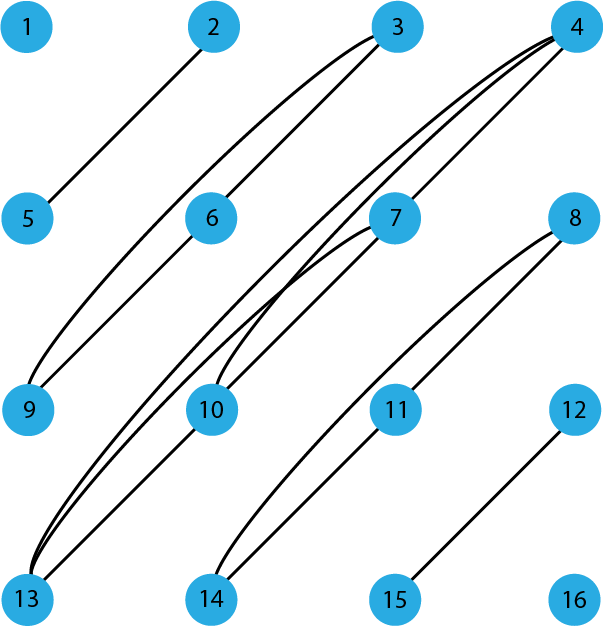
\includegraphics[width=0.5\textwidth]{images/anti_diag_square_constraint.png}
	\caption{Minh họa liên kết các ô trong ràng buộc đường chéo phụ với N = 4 trong công thức bình phương}
	\label{fig:anti-diag-square-constraint}
\end{figure}


\textbf{Bước 4: Kết hợp biểu thức}
\[
H =H_{obj}+\lambda_1 H_1+\lambda_2 H_2+\lambda_3 H_3+\lambda_4 H_4
\]

\[
	H =
	\lambda_1 \sum_{u}^{}{(1-\sum{}^{}{R_u})^2} + 
	\lambda_2 \sum_{u}^{}{(1-\sum{}^{}{C_u})^2} +
	\lambda_3 \sum_{u}^{}{( \sum_{i<j}^{}{D_{ui}D_{uj}})} +
	\lambda_4 \sum_{u}^{}{( \sum_{i<j}^{}{A_{ui}A_{uj}})}
\]

\textbf{Triển khai thuật toán:}


\begin{algorithm}[H]
    \caption{[Bình phương] Biểu thị mỗi ô trên bàn cờ bằng một tập hợp con các ID ràng buộc.}
    \begin{algorithmic}[1]
   	
    \Function{Build\_Subsets}{$n$}
	
        \State $subsets \gets \text{empty list}$
        \For{$x \text{ in range }(n)$}
            \For{$y \text{ in range }(n)$}
                \State $col \gets x$ 
                \State $row \gets y + n$ 
                \State $subset \gets \{col, row\}$
                \State $diag \gets x + y + (2*n - 1)$ 
                \State $min\_diag \gets 2*n$
                \State $max\_diag \gets 4*  n - 4$
                \If{$diag \geq min\_diag \text{ and } diag \leq max\_diag$}
                    \State $subset.add(diag)$
                \EndIf
                \State $anti\_diag \gets (n - 1 - x + y) + (4*n - 4)$ 
                
                \State $min\_anti\_diag \gets 4*n - 3$
                \State $max\_anti\_diag \gets 6*n - 7$
                \If{$anti\_diag \geq min\_anti\_diag \text{ and } anti\_diag \leq max\_anti\_diag$}
                    \State $subset.add(anti\_diag)$
                \EndIf
                \State $subsets.append(subset)$
            \EndFor
        \EndFor
        \State \Return $subsets$
    \EndFunction
    \end{algorithmic}
\end{algorithm}


Trong đó, hàm \textsc{Build\_Subsets} trả về danh sách các tập hợp con của các ràng buộc tương ứng với mọi ô trên bàn cờ. Mỗi ràng buộc được biểu thị bằng một số duy nhất (ID). Mỗi tập hợp con sẽ chứa:
\begin{enumerate}
	

	\item Chính xác một ID ràng buộc cột (0 đến n-1).
	\item Chính xác là một ID ràng buộc hàng (n đến 2*n-1).
	\item Tối đa một ID ràng buộc theo đường chéo chính (trên cùng bên trái đến dưới cùng bên phải) (4*n-3
	đến 6*n-7).
	\item Tối đa một ID ràng buộc theo đường chéo phụ (từ dưới cùng bên trái đến trên cùng bên phải) (2*n đến
	4*n-4).
\end{enumerate}
\begin{algorithm}[H]
	\caption{[Bình phương] Xây dựng mô hình bậc hai nhị phân sử dụng các tập hợp con ràng buộc}
    \begin{algorithmic}[1]
        \Function{exact\_cover\_bqm}{$problem\_set, subsets$}
            \State $bqm \gets \text{BinaryQuadraticModel}(\{\}, \{\}, 0, 'BINARY')$
            \State $cnt \gets 0$
            \For{$element$ in $problem\_set$}
                \State $bqm.offset \gets bqm.offset + 1$
                \For{$i$ in range(len($subsets$))}
                    \If{$element$ in $subsets[i]$}
                        \State $bqm.add\_variable(i, -1)$
                        \For{$j$ in range($i$)}
                            \If{$element$ in $subsets[j]$}
                                \State $bqm.add\_interaction(i, j, 2)$
                            \EndIf
                        \EndFor
                    \EndIf
                \EndFor
            \EndFor
            \State \Return $bqm$
        \EndFunction
        \State
        \Function{handle\_diag\_constraints}{$bqm, subsets, diag\_constraints$}
            \For{$constraint$ in $diag\_constraints$}
                \For{$i$ in range(len($subsets$))}
                    \If{$constraint$ in $subsets[i]$}
                        \For{$j$ in range($i$)}
                            \If{$constraint$ in $subsets[j]$}
                                \State $bqm.add\_interaction(i, j, 2)$
                            \EndIf
                        \EndFor
                    \EndIf
                \EndFor
            \EndFor
            \State \Return $bqm$
        \EndFunction
            
    \end{algorithmic}
    
\end{algorithm}

Áp dụng từ bài toán bao phủ chính xác vào ràng buộc hàng và cột, ta có hàm \textsc{exact\_cover\_bqm} trả về một mô hình bậc hai nhị phân cho một tập hợp các tập hợp con của problem\_set chứa mọi phần tử trong problem\_set đúng một lần. Hàm \textsc{handle\_diag\_constraints} cập nhật mô hình với các ràng buộc đường chéo chính (và đường chéo phụ). Nếu trùng lặp sẽ bị phạt.

\begin{algorithm}[H]
	\caption{Lấy mẫu}
	\begin{algorithmic}[1]
		
		\State $sampler \gets \text{EmbeddingComposite(DWaveSampler())}$
		\State $num\_reads \gets 1000$
		\State $sampleset \gets \text{sampler.sample(bqm, num\_reads=num\_reads)}$
		
	\end{algorithmic}
	
\end{algorithm}

Sau khi đã ánh xạ các ràng buộc vào mô hình bậc hai nhị phân, chúng ta sẽ lấy mẫu, là một tập hợp các lời giải tiềm năng chứa tập các ID ràng buộc biểu thị các ô đặt quân hậu.

\begin{algorithm}[H]
    \caption{Kiểm tra lời giải}
    \begin{algorithmic}[1]
        \Function{is\_valid\_solution}{$n, solution$}
            %\Comment{Check that solution is valid by making sure all constraints were met.}
            \State $count \gets \text{Counter}()$
            \For{$queen$ in $solution$}
                \State $count \gets count + \text{Counter}(queen)$
            \EndFor
            %\Comment{Check row/col constraints}
            \For{$i$ in range($2*n$)}
                \If{$count[i] \neq 1$}
                    \If{$i < n$}
                        \State $col \gets i$
                        \State \text{print}("Column {} has {} queens.".format($col, count[i]$))
                    \Else
                        \State $row \gets np.abs(i - (2*n - 1))$ %\Comment{Convert constraint id to row index}
                        \State \text{print}("Row {} has {} queens.".format($row, count[i]$))
                    \EndIf
                    \State \Return False
                \EndIf
            \EndFor
%            \Comment{Check diag/anti-diag constraints}
            \For{$i$ in range($2*n, 4*n - 6$)}
                \If{$count[i] > 1$}
                    \If{$i \leq 4*n - 4$}
                        \State \text{print}("Top-left to bottom-right diagonal {} has {} queens.".format($i, count[i]$))
                    \Else
                        \State \text{print}("Bottom-left to top-right diagonal {} has {} queens.".format($i, count[i]$))
                    \EndIf
                    \State \Return False
                \EndIf
            \EndFor
            \State \Return True
        \EndFunction
    \end{algorithmic}
\end{algorithm}
    
    Sau khi lấy mẫu, chúng ta sẽ kiểm tra xem lời giải có hợp lệ hay không bằng cách đảm bảo đáp ứng tất cả các ràng buộc.

\subsection{Công thức cộng dồn cho bài toán xếp hậu}

So với công thức bình phương, thì công thức cộng dồn có phần khác biệt trong cách thêm biến phụ và liên kết giữa các biến 
nên chúng ta sẽ có thay đổi ở bước 3 và bước 4.

\textbf{Bước 3: Chuyển đổi biểu thức toán học thành mô hình bậc hai nhị phân}

Ràng buộc 1: Có chính xác một quân hậu trên mỗi hàng. (Hình \ref{fig:row-square-constraint})

\[
H_1 = \sum_{u}^{}{(1-\sum{}^{}{R_u})^2}
\]


Ràng buộc 2: Có chính xác một quân hậu trên mỗi cột. (Hình \ref{fig:col-square-constraint})

\[
H_2 = \sum_{u}^{}{(1-\sum{}^{}{C_u})^2}
\]

Ràng buộc 3: Có nhiều nhất một quân hậu nằm trên mỗi đường chéo chính (từ trên cùng bên trái đến dưới cùng bên phải).


Với mỗi tập $D_u$ có $D_{ui}, D_{uj}$ tương ứng là phần tử thứ i, j của tập $D_u$, ta thêm tập các biến phụ (biến nhị phân) $S_{u}^{D} $ có $S_{ui}^{D}, S_{uj}^{D}$ tương ứng là phần tử thứ i, j của tập $S_{u}^{D}$. Ta có:

\[
H_3 = \sum_{u}^{}{\left[ (S_{u1}^{D} - D_{u1} - D_{u2})^2 + \sum_{i=2}^{}{(S_{ui}^{D} - S_{u(i-1)}^{D} - D_{u(i+1)})^2}  \right]}
\]

\begin{figure}[H]
	\centering
	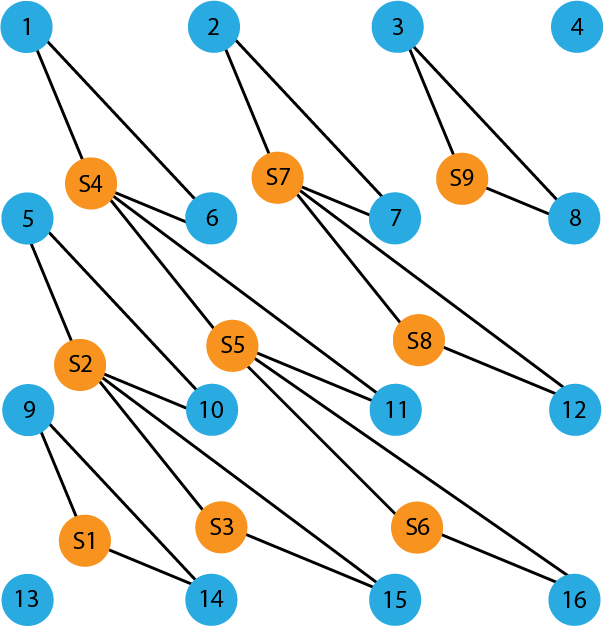
\includegraphics[width=0.5\textwidth]{images/main_diag_add_constraint.png}
	\caption{Minh họa liên kết các ô trong ràng buộc đường chéo chính với N = 4 trong công thức cộng dồn}
\end{figure}

Ràng buộc 4: Có nhiều nhất một quân hậu nằm trên mỗi đường chéo phụ (từ dưới cùng bên trái đến trên cùng bên phải).

Với mỗi tập $A_u$ có $A_{ui}, A_{uj}$ tương ứng là phần tử thứ i, j của tập $A_u$, ta thêm tập các biến phụ (biến nhị phân) $S_u^A $ có $S_{ui}^{A}, S_{uj}^{A}$ tương ứng là phần tử thứ i, j của tập $S_u^A$. Ta có:

\[
H_4 = \sum_{u}^{}{\left[ (S_{u1}^{A} - A_{u1} - A_{u2})^2 + \sum_{i=2}^{}{(S_{ui}^{A} - S_{u(i-1)}^{A} - A_{u(i+1)})^2}  \right]}
\]
\begin{figure}[H]
	\centering
	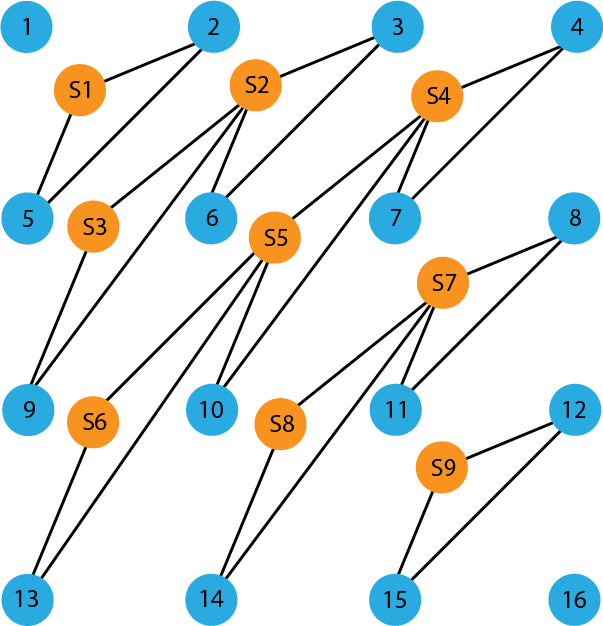
\includegraphics[width=0.5\textwidth]{images/anti_diag_add_constraint.png}
	\caption{Minh họa liên kết các ô trong ràng buộc đường chéo phụ với N = 4 trong công thức cộng dồn}
\end{figure}
\textbf{Bước 4: Kết hợp biểu thức}
\[
H =H_{obj}+\lambda_1 H_1+\lambda_2 H_2+\lambda_3 H_3+\lambda_4 H_4
\]


\begin{multline*}
	H =
	\lambda_1 \sum_{u}^{}{(1-\sum{}^{}{R_u})^2} + 
	\lambda_2 \sum_{u}^{}{(1-\sum{}^{}{C_u})^2} + \\
	\lambda_3 \sum_{u}^{}{\left[ (S_{u1}^{D} - D_{u1} - D_{u2})^2 + \sum_{i=2}^{}{(S_{ui}^{D} - S_{u(i-1)}^{D} - D_{u(i+1)})^2}  \right]} + \\
	\lambda_4 \sum_{u}^{}{\left[ (S_{u1}^{A} - A_{u1} - A_{u2})^2 + \sum_{i=2}^{}{(S_{ui}^{A} - S_{u(i-1)}^{A} - A_{u(i+1)})^2}  \right]}
 \nonumber
\end{multline*}

\textbf{Triển khai thuật toán:}

\begin{algorithm}[H]
    \caption{[Cộng dồn] Biểu thị mỗi ô trên bàn cờ bằng một tập hợp các ID}
    \begin{algorithmic}
    \For{$i$ in range($n$)}
        \State $s[i] \gets \text{dict}()$
        \For{$j$ in range($n$)}
            \State $s[i][j] \gets i \times n + j$
%            \State $varnames.append("X\{" + \text{str}(i) + "," + \text{str}(j) + "\}")$
%            \State $NumVar += 1$
        \EndFor
    \EndFor
    \State
    \State dia = \text{dict}()
    
    \For{$i$ in range($n$)}
    \For{$j$ in range($n$)}
    \If{$(i + j)$ not in dia}
    \State    dia[$i + j$] = [s[$i$][$j$]]
    \Else
    \State    dia[$i + j$].append(s[$i$][$j$])
    \EndIf
    \EndFor
    \EndFor
    
    
    \State
    \State rdia = \text{dict}()
    \For{$i$ in range($n$)}
    \For{$j$ in range($n$)}
    \If{$(i - j)$ not in rdia}
    \State rdia[$i - j$] = [s[$i$][$j$]]
    \Else
    \State rdia[$i - j$].append(s[$i$][$j$])
    \EndIf
    \EndFor
    \EndFor
    \end{algorithmic}
\end{algorithm}
    Chúng ta xây dựng một tập hợp các ID tương ứng với mọi ô trên bàn cờ theo hướng từ trái sang phải, từ trên xuống dưới, được đánh số từ 0 đến $n^2 -1$.


\begin{algorithm}[H]
    \caption{[Cộng dồn] Xây dựng mô hình bậc hai nhị phân cho ràng buộc hàng và ràng buộc cột}
    \begin{algorithmic}[1]
    \Function {exact\_cover\_bqm}{bqm, variables}:
    \State  bqm.offset += 1
    \For {i, var in enumerate(variables)}
    \State   bqm.add\_variable(var, -1)
    \For{j in range(i)}
    \State    bqm.add\_interaction(variables[j], var, 2)
       \EndFor
    \EndFor
%    \State  \Return
	
    \EndFunction
    \State
    \For{$i$ in range($n$)}
    \State  vars $\gets$ []
    \For{$j$ in range($n$)}
    \State   bqm.add\_variable(s[i][j], -1)
    \State   vars.append(s[i][j])
    \EndFor
    \State  exact\_cover\_bqm(bqm, vars)
    \State  vars $\gets$ []
    \For{$j$ in range($n$)}
    \State   vars.append(s[j][i])
    \EndFor
    \State  exact\_cover\_bqm(bqm, vars)
    \EndFor
    \end{algorithmic}
\end{algorithm}
    Chúng ta xây dựng mô hình bậc hai nhị phân cho ràng buộc hàng và cột. Và tiếp bên dưới, chúng ta cập nhật mô hình bậc hai nhị phân cho ràng buộc đường chéo chính và đường chéo phụ cho công thức cộng dồn của chúng ta.

\begin{algorithm}[H]
	\caption{[Cộng dồn] Xây dựng mô hình bậc hai nhị phân cho ràng buộc đường chéo chính và phụ}
	\begin{algorithmic}[1]
		
		\Function {add\_constraint}{bqm, S, x1, x2}:
		\State  $\lambda = 3$
		\State  bqm.add\_variable(S, $\lambda \times (1 / 2)$)
		\State  bqm.add\_variable(x1, $\lambda \times (1 / 2)$)
		\State  bqm.add\_variable(x2, $\lambda \times (1 / 2)$)
		\State  bqm.add\_interaction(S, x1, $\lambda \times (-1)$)
		\State  bqm.add\_interaction(S, x2, $\lambda \times (-1)$)
		\State  bqm.add\_interaction(x1, x2, $\lambda \times 2$)
		\EndFunction
		
		\State
		\State NumVar = $n \times n$
		\Function {dia\_constraints\_bqm}{bqm, subsetDict, type}:
		\For{k, subset\_indices in subsetDict.items()}
		\If{len(subset\_indices) $\leq$ 1}
		\State    \textbf{continue}
		\EndIf
		\State   key = type + str(k)
		\If{key not in s}
		\State    s[key] = \{\}
		\EndIf
		\State   s[key][0] = NumVar
		\State   add\_constraint(bqm, NumVar, subset\_indices[0], subset\_indices[1])
		\State   NumVar += 1
		\For{i in range(2, len(subset\_indices))}
		\State    s[key][i - 1] = NumVar
		\State    add\_constraint(bqm, NumVar, s[key][i - 2], subset\_indices[i])
		\State    NumVar += 1
		\EndFor
		\EndFor
		\EndFunction
		
		\State
		\State dia\_constraints\_bqm(bqm, dia, '+')
		\State dia\_constraints\_bqm(bqm, rdia, '-')
        
	\end{algorithmic}
\end{algorithm}



\chapter{Thực nghiệm}
Mục tiêu thử nghiệm là minh họa sự so sánh giữa phương pháp được đề xuất bởi D-wave với phương pháp cải tiến của chúng ta nhằm xây dựng lại bài toán xếp hậu dựa trên mô hình bậc hai nhị phân.
\section{Cài đặt}
\subsection{Hệ thống}
Tất cả các thí nghiệm ủ lượng tử đều được thực hiện trên D-Wave Advantage, công cụ ủ lượng tử mới nhất do D-Wave System Inc trình bày. Phiên bản được sử dụng là Advantage System 4.1, tính toán lượng tử đoạn nhiệt dựa trên kiến trúc Pegasus với 5627 hạt lượng tử hoạt động. \cite{Performance Update} 
\subsection{Phương pháp}
Chúng ta sẽ chạy thử nghiệm so sánh các phương pháp sử dụng mô hình bậc hai nhị phân được thảo luận ở trên  bao gồm công thức bình phương do D-Wave đề xuất và công thức cộng dồn là công thức cải tiến của chúng ta.
%	\section{Parameters}

\subsection{Số liệu} 

Đối với mỗi công thức, chúng ta ghi lại số lượng biến ($\#Var$), số tương tác giữa các biến trong công thức QUBO($\#Interaction$), số lượng hạt lượng tử vật lý($\#Qubit$), tỷ lệ phần trăm các trường hợp trong đó một lời giải tối ưu được tìm thấy ($\%Sol$). 

$\%OptGap$ là khoảng cách từ lời giải tốt nhất tìm được tới lời giải tối ưu:
\[
	\%OptGap = \frac{n - n_{best}}{n}
\]
trong đó: n là số hậu cần đặt, $n_{best}$ là số hậu tốt nhất trong $\alpha$ lần chạy.

$TTS(t_f)$ là thời gian tìm ra được một lời giải với xác suất kỳ vọng là $N_{exp}$:

$$TTS(t_f) = t_f \cdot N_{exp}$$

trong đó: 
 $t_f$ là thời gian chạy trung bình của một lần đọc có tính đến thời gian lập trình ban đầu ($t_{prog}$), thời gian ủ ($t_{annealing}$) và thời gian đọc ( $t_{readout}$) cho mỗi mẫu:
		
		$$t_f = \frac{t_{prog}}{N_{read}} + t_{annealing} + t_{readout}$$
, $N_{exp}$ là xác suất kỳ vọng:
$$N_{exp} = \frac{1}{\%Sol}$$
Do đó, nó không bao gồm thời gian truy cập và thời gian nhúng QUBO vào biểu đồ phần cứng.

\section{Kết quả}

	\subsection{So sánh giữa các công thức }
	
	\begin{table}[H]
		\centering
		\begin{tabular}{ c c c c c c}
			\hline
			Công thức & \textbf{Bình phương} & \textbf{Cộng dồn} \\
			\hline
			\textbf{$\#Var$}     & $N^2$ & $3N^2 - 4N + 2$ \\
			\textbf{$\#Interaction$}     & $\frac{5}{3}N^3 - 2N^2 + \frac{N}{3}$ & $N^3 + 5N^2 -12N +6$\\
			
			\hline
		\end{tabular}
		\caption{Bảng công thức tính số lượng biến và số liên kết sử dụng trong công thức bình phương và công thức cộng dồn theo số quân hậu}
		\label{tab:var_and_interaction}
	\end{table}
	
		
	\begin{table}[H]
		\centering
		\begin{tabular}{|c|c|c|c|c|c|c|c|c|c|c|c|c|c|c|}
			\hline
			N & 4 & 5 & 6 & 7 & 8 & 9 & 10 & 11 & 12 & 13 & 14 & 15 & 16 \\
			\hline
			Bình phương & 16 & 25 & 36 & 49 & 64 & 81 & 100 & 121 & 144 & 169 & 196 & 225 & 256 \\
			\hline
			Cộng dồn & 34 & 57 & 86 & 121 & 162 & 209 & 262 & 321 & 386 & 457 & 534 & 617 & 706 \\
			\hline
		\end{tabular}
		
		
		
		\caption{Bảng số lượng biến sử dụng trong công thức bình phương và công thức cộng dồn theo số quân hậu}
		\label{tab:var_num}
	\end{table}
	
	\begin{figure}[H]
		\centering
		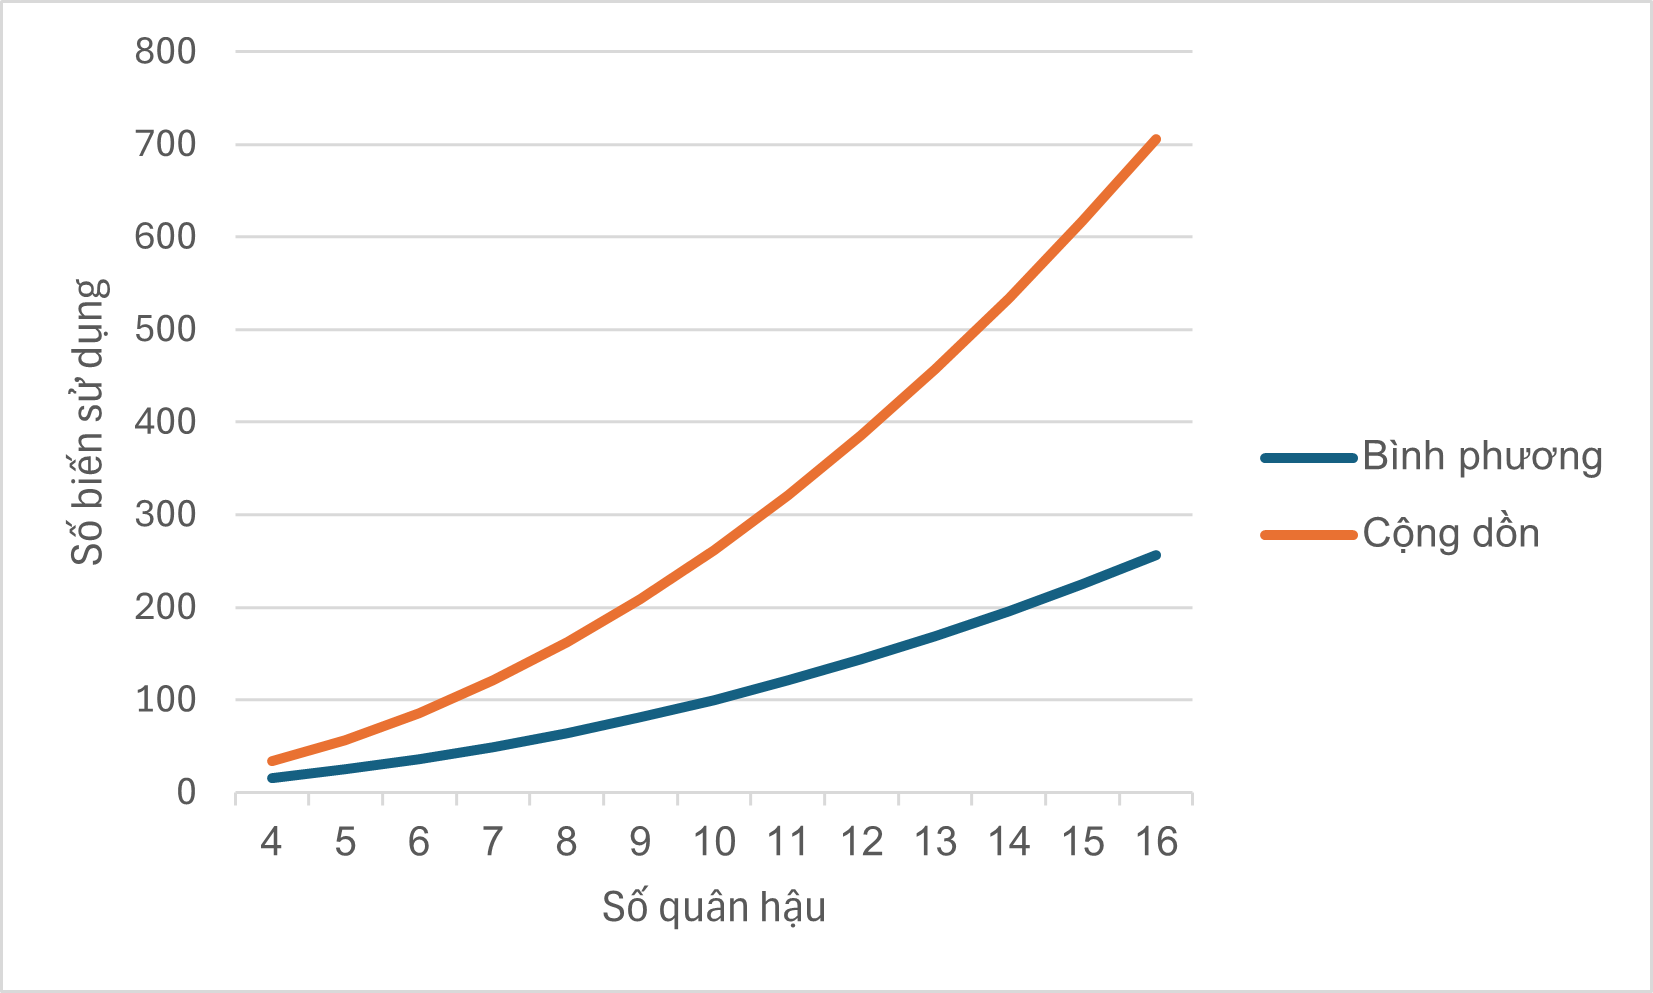
\includegraphics[width=0.7\textwidth]{images/methods/var_num.png}
		\caption{Biểu đồ số lượng biến sử dụng trong công thức bình phương và công thức cộng dồn theo số quân hậu}
		\label{fig:var_num}
	\end{figure}
	
	\begin{table}[H]
		\centering
		\begin{tabular}{|c|c|c|c|c|c|c|c|c|c|c|c|c|c|c|}
			\hline
			N & 4 & 5 & 6 & 7 & 8 & 9 & 10 & 11 & 12 & 13 & 14 & 15 & 16 \\
			\hline
			Bình phương & 76 & 160 & 290 & 476 & 728 & 1056 & 1470 & 1980 & 2596 & 3328 & 4186 & 5180 & 6320 \\
			\hline
			Cộng dồn & 102 & 196 & 330 & 510 & 742 & 1032 & 1386 & 1810 & 2310 & 2892 & 3562 & 4326 & 5190 \\
			\hline
		\end{tabular}
		
		
		
		\caption{Bảng số lượng tương tác giữa các biến trong công thức bình phương và công thức cộng dồn theo số quân hậu}
		\label{tab:interaction_num_cmp}
	\end{table}
	
	\begin{figure}[H]
		\centering
		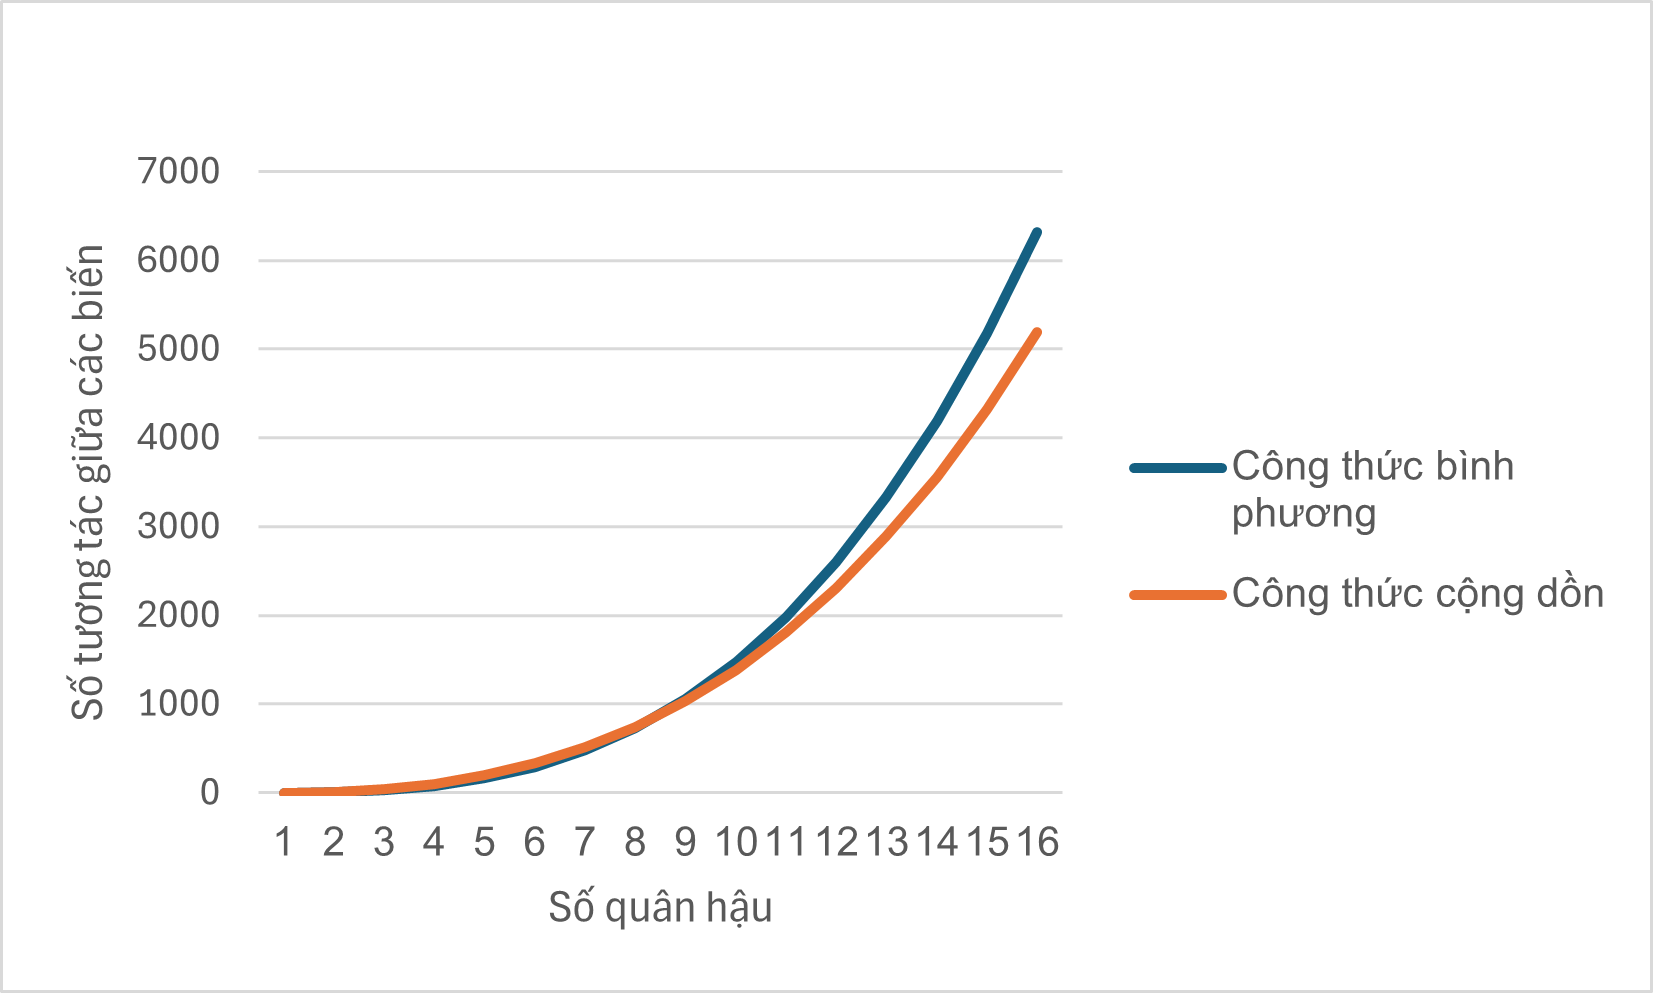
\includegraphics[width=0.7\textwidth]{images/interaction_num_cmp.png}
		\caption{Biểu đồ số lượng tương tác giữa các biến trong công thức bình phương và công thức cộng dồn theo số quân hậu }
		\label{fig:interaction_num_cmp}
	\end{figure}
	Như được hiển thị trong hình~\ref{fig:var_num}, do công thức cộng dồn cần sử dụng thêm biến phụ nên dễ dàng nhận thấy số lượng biến cần dùng của công thức bình phương luôn luôn ít hơn của công thức cộng dồn. Tuy nhiên, từ hình~\ref{fig:interaction_num_cmp} có thể thấy ban đầu số lượng liên kết công thức cộng dồn sử dụng vẫn nhỉnh hơn chút với đầu vào số quân hậu nhỏ, nhưng khi số quân hậu dần tăng lên thì công thức cộng dồn lại chiếm ưu thế so với công thức bình phương.


\begin{table}[H]
	\centering
	\begin{tabular}{|c|c|c|c|c|c|c|c|c|c|c|}
		\hline
		N & 4 & 5 & 6 & 7 & 8 & 9 & 10 & 11 & 12 & 13 \\
		\hline
		Bình phương & 32.{6} & 73 & 146.{3} & 264.{3} & 450.{6} & 759.{3} & 1187.{3} & 1708 & 2540.{3} & 3558.{6} \\
		\hline
		Cộng dồn & 63.{3} & 135 & 244 & 446.{3} & 704.{6} & 1086 & 1723.{3} & 2535 & 3249.{3} & 4167.{3} \\
		\hline
	\end{tabular}
	\caption{Bảng số lượng hạt lượng tử vật lý cần dùng trong công thức bình phương và công thức cộng dồn theo số quân hậu}
	\label{tab:num_qubit}
\end{table}

\begin{figure}[H]
	\centering
	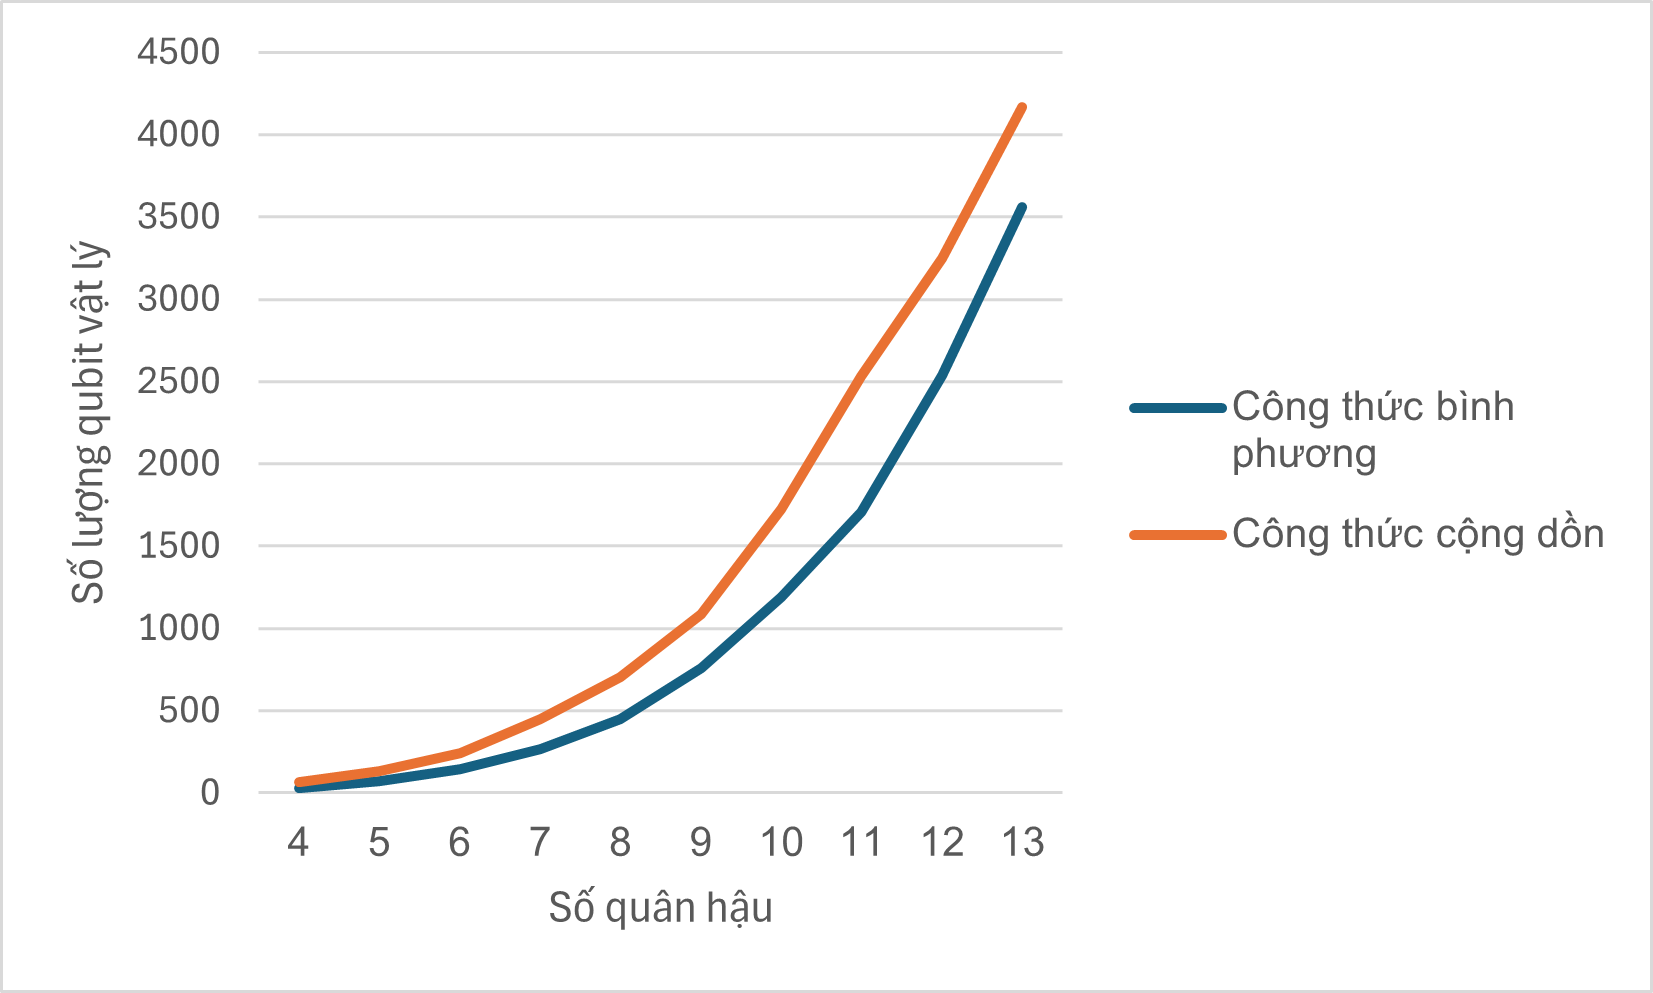
\includegraphics[width=0.7\textwidth]{images/methods/num_qubit.png}
	\caption{Biểu đồ số lượng hạt lượng tử vật lý cần dùng trong công thức bình phương và công thức cộng dồn theo số quân hậu}
	\label{fig:num_qubit}
\end{figure}


\begin{table}[H]
	\centering
	\begin{tabular}{|c|c|c|c|c|c|c|c|c|c|c|}
		\hline
		N & 4 & 5 & 6 & 7 & 8 & 9 & 10 & 11 & 12 & 13 \\
		\hline
		Bình phương & 85.53 & 58.1 & 4.6 & 2.8 & 0 & 0 & 0 & 0 & 0 & 0 \\
		\hline
		Cộng dồn & 25.63 & 10.43 & 0.07 & 0.03 & 0 & 0 & 0 & 0 & 0 & 0 \\
		\hline
	\end{tabular}
	
	\caption{Bảng tỷ lệ phần trăm lời giải tối ưu được tìm thấy ($\%sol$) trong công thức bình phương và công thức cộng dồn theo số quân hậu}
	\label{tab:methods/sol}
\end{table}

\begin{figure}[H]
	\centering
	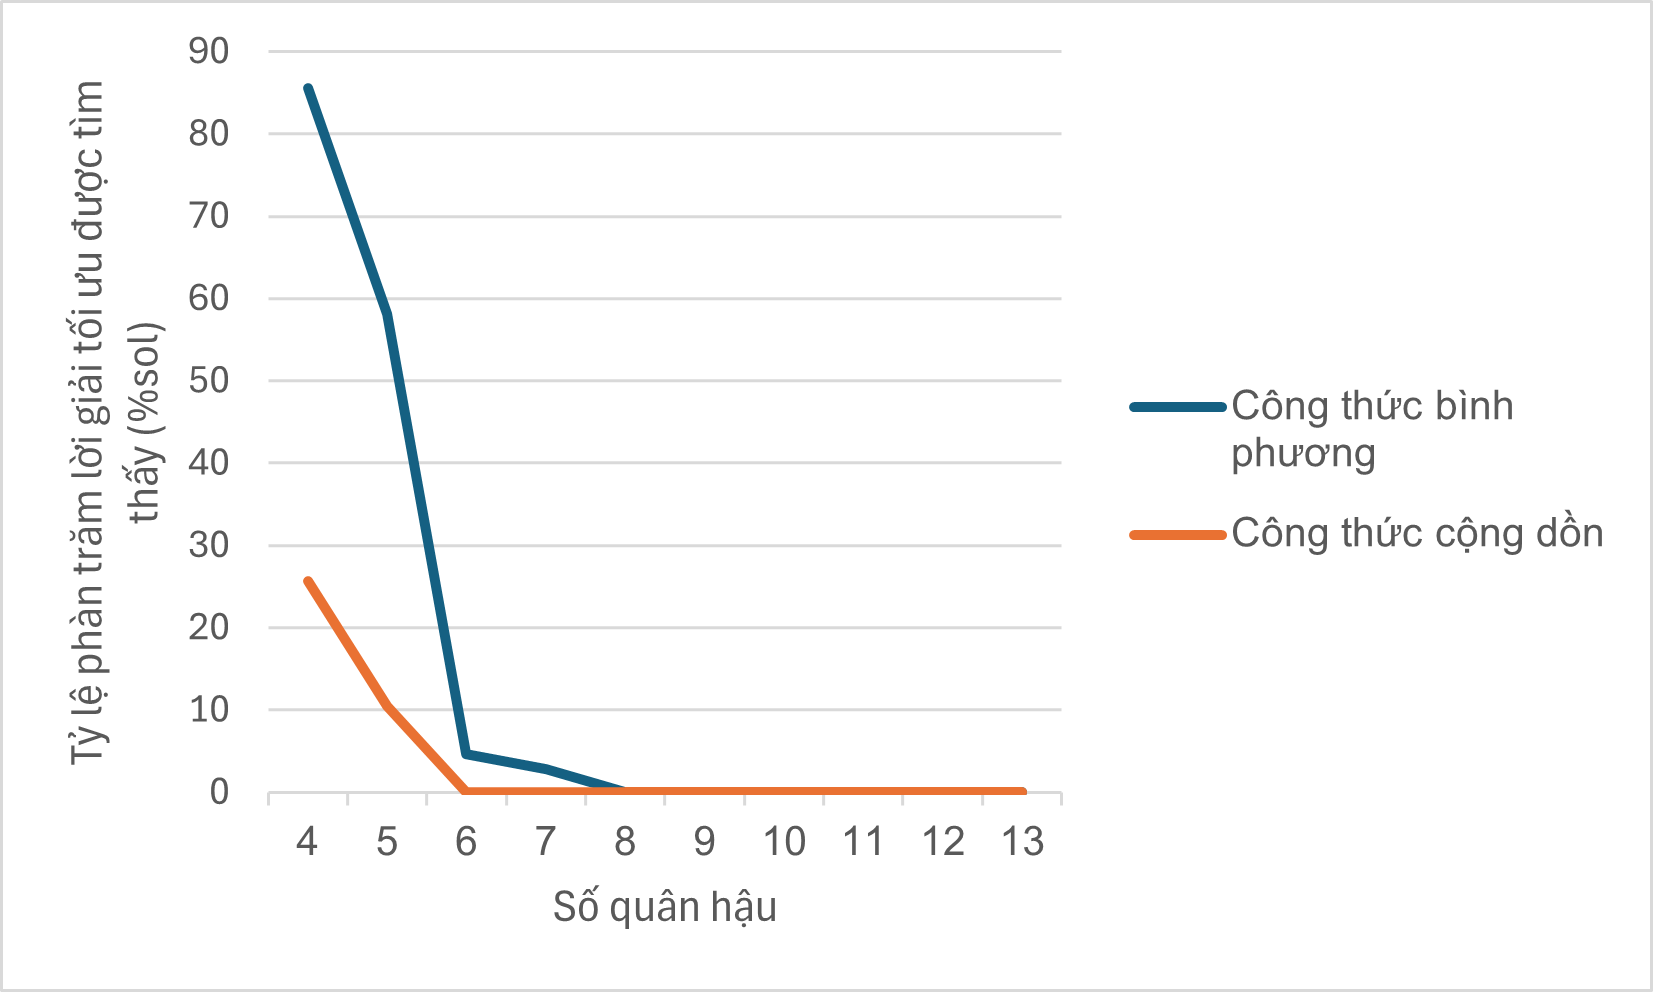
\includegraphics[width=0.7\textwidth]{images/methods/sol.png}
	\caption{Biểu đồ tỷ lệ phần trăm lời giải tối ưu tìm được ($\%sol$) trong công thức bình phương và công thức cộng dồn theo số quân hậu}
	\label{fig:methods/sol}
\end{figure}

Tuy công thức cộng dồn làm giảm bớt số liên kết giữa các biến nhưng việc tăng số lượng biến vẫn cho thấy số lượng hạt lượng tử cần dùng không những không giảm mà còn cần dùng nhiều hơn (Hình~\ref{fig:num_qubit}). Thêm vào đó, tỷ lệ phần trăm lời giải tối ưu được tìm thấy cũng giảm theo (Hình~\ref{fig:methods/sol}).

\begin{table}[H]
	\centering
	\begin{tabular}{|c|c|c|c|c|c|c|c|c|c|c|}
		\hline
		N & 4 & 5 & 6 & 7 & 8 & 9 & 10 & 11 & 12 & 13 \\
		\hline
		Bình phương & 0 & 0 & 0 & 0 & 4.16 & 7.41 & 20 & 18.18 & 22.22 & 25.64 \\
		\hline
		Cộng dồn & 0 & 0 & 0 & 0 & 4.17 & 14.81 & 6.67 & 18.18 & 30.55 & 25.64 \\
		\hline
	\end{tabular}
	
	
	\caption{Bảng khoảng cách từ lời giải tốt nhất tìm được tới lời giải tối ưu ($\%OptGap$) trong công thức bình phương và công thức cộng dồn theo số quân hậu}
	\label{tab:methods/optgap}
\end{table}

\begin{figure}[H]
	\centering
	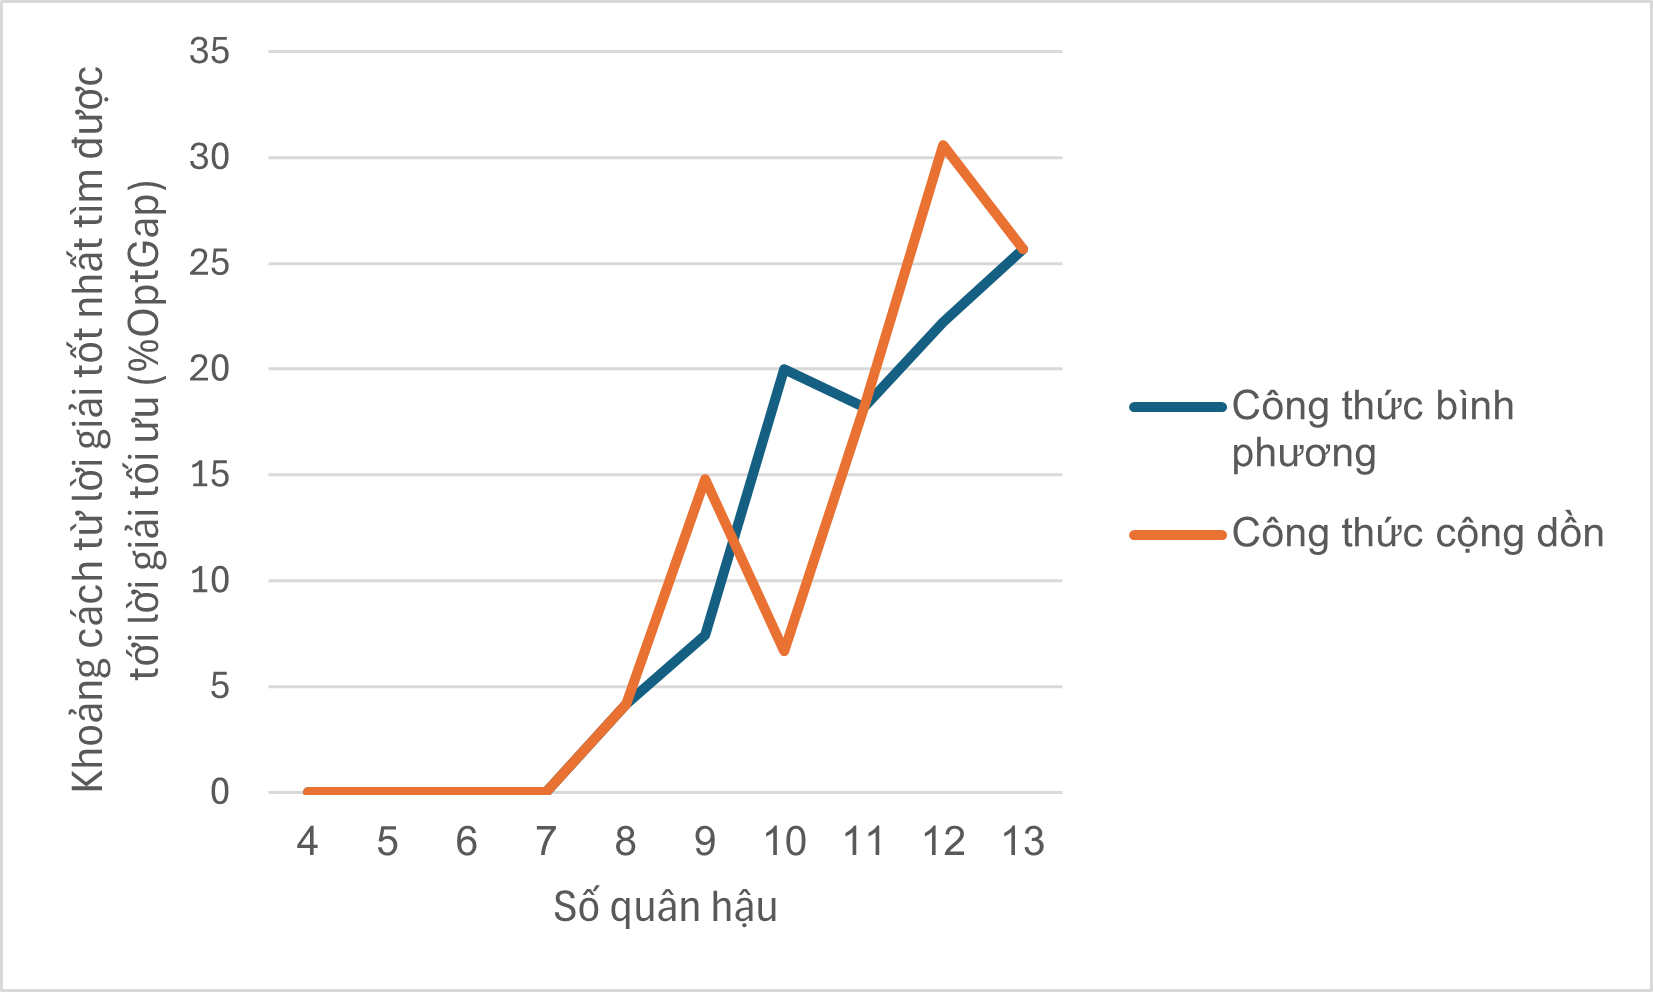
\includegraphics[width=0.7\textwidth]{images/methods/optgap.png}
	\caption{Biểu đồ khoảng cách từ lời giải tốt nhất tìm được tới lời giải tối ưu ($\%OptGap$) trong công thức bình phương và công thức cộng dồn theo số quân hậu}
	\label{fig:methods/optgap}
\end{figure}

Với điều kiện tiên quyết là giảm bớt số liên kết và chỉ cần lời giải gần đúng thì hình~\ref{fig:methods/optgap} cho thấy công thức cộng dồn vẫn coi là chấp nhận được, tuy rằng $\%OptGap$ có dao động đôi chút.

	\subsection{So sánh với ủ mô phỏng}
	
		\begin{table}[H]
		\centering
		\begin{tabular}{|c|c|c|c|c|c|c|c|c|c|c|}
			\hline
			N & 4 & 5 & 6 & 7 & 8 & 9 & 10 & 11 & 12 & 13 \\
			\hline
			Ủ lượng tử & 0.12 & 0.14 & 0.19 & 0.19 & 0.15 & 0.19 & 0.21 & 0.23 & 0.25 & 0.27 \\
			\hline
			Ủ mô phỏng & 0.23 & 0.39 & 0.58 & 0.81 & 1.05 & 1.37 & 1.78 & 2.24 & 2.76 & 3.3 \\
			\hline
		\end{tabular}
		
		
		\caption{Bảng thời gian chạy trung bình của một lần đọc (ms)  của ủ lượng tử và ủ mô phỏng theo số quân hậu}
		\label{tab:SA_QA/t_f}
	\end{table}
	
	\begin{figure}[H]
		\centering
		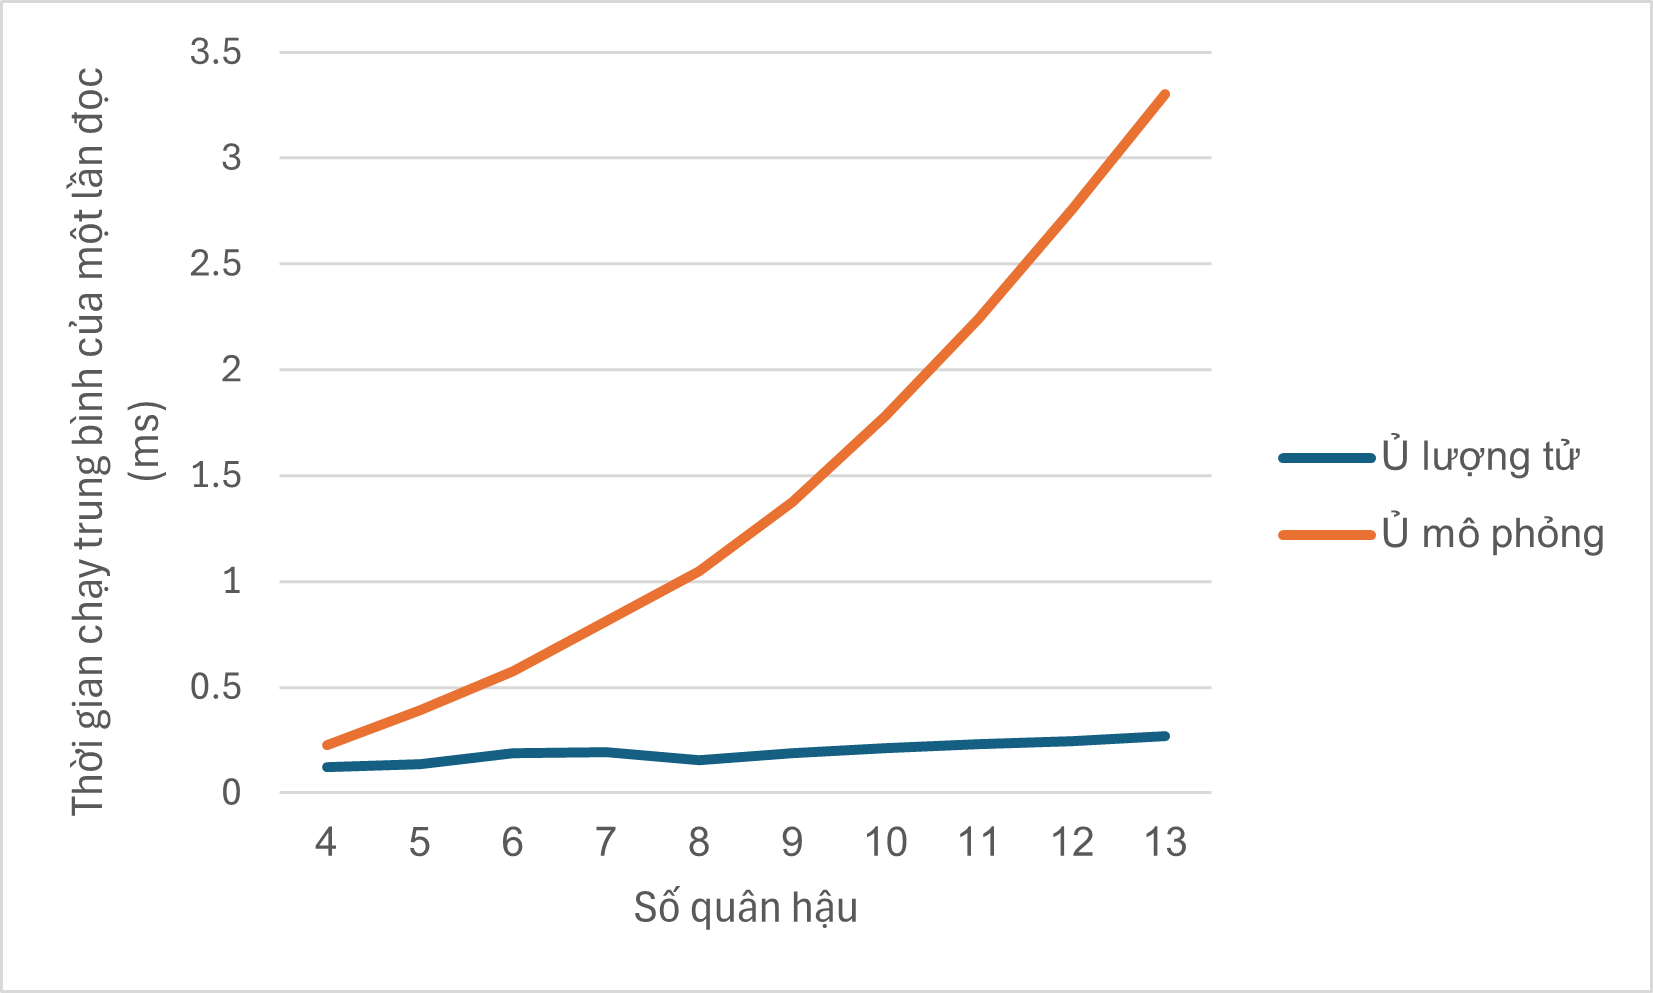
\includegraphics[width=0.7\textwidth]{images/SA_QA/t_f.png}
		\caption{Biểu đồ thời gian chạy trung bình của một lần đọc (ms)  của ủ lượng tử và ủ mô phỏng theo số quân hậu}
		\label{fig:SA_QA/t_f}
	\end{figure}
	Hình \ref{fig:SA_QA/t_f} đã chỉ ra độ phức tạp về thời gian có tác động lớn đối với quá trình ủ mô phỏng và nó không phải là hằng số. Ngược lại, quá trình ủ lượng tử thực sự có độ phức tạp về thời gian không đổi.
	
		\begin{table}[H]
		\centering
		\begin{tabular}{|c|c|c|c|c|c|c|c|c|c|c|}
			\hline
			N & 4 & 5 & 6 & 7 & 8 & 9 & 10 & 11 & 12 & 13 \\
			\hline
			Ủ lượng tử & 85.53 & 58.1 & 4.6 & 2.8 & 0 & 0 & 0 & 0 & 0 & 0 \\
			\hline
			Ủ mô phỏng & 100 & 100 & 97.6 & 98.93 & 99.67 & 99.7 & 99.47 & 99.4 & 99.67 & 99.67 \\
			\hline
		\end{tabular}
		
		
		\caption{Bảng tỷ lệ phần trăm lời giải tối ưu được tìm thấy ($\%sol$)  của ủ lượng tử và ủ mô phỏng theo số quân hậu}
		\label{tab:SA_QA/sol}
	\end{table}
	
	
	\begin{figure}[H]
		\centering
		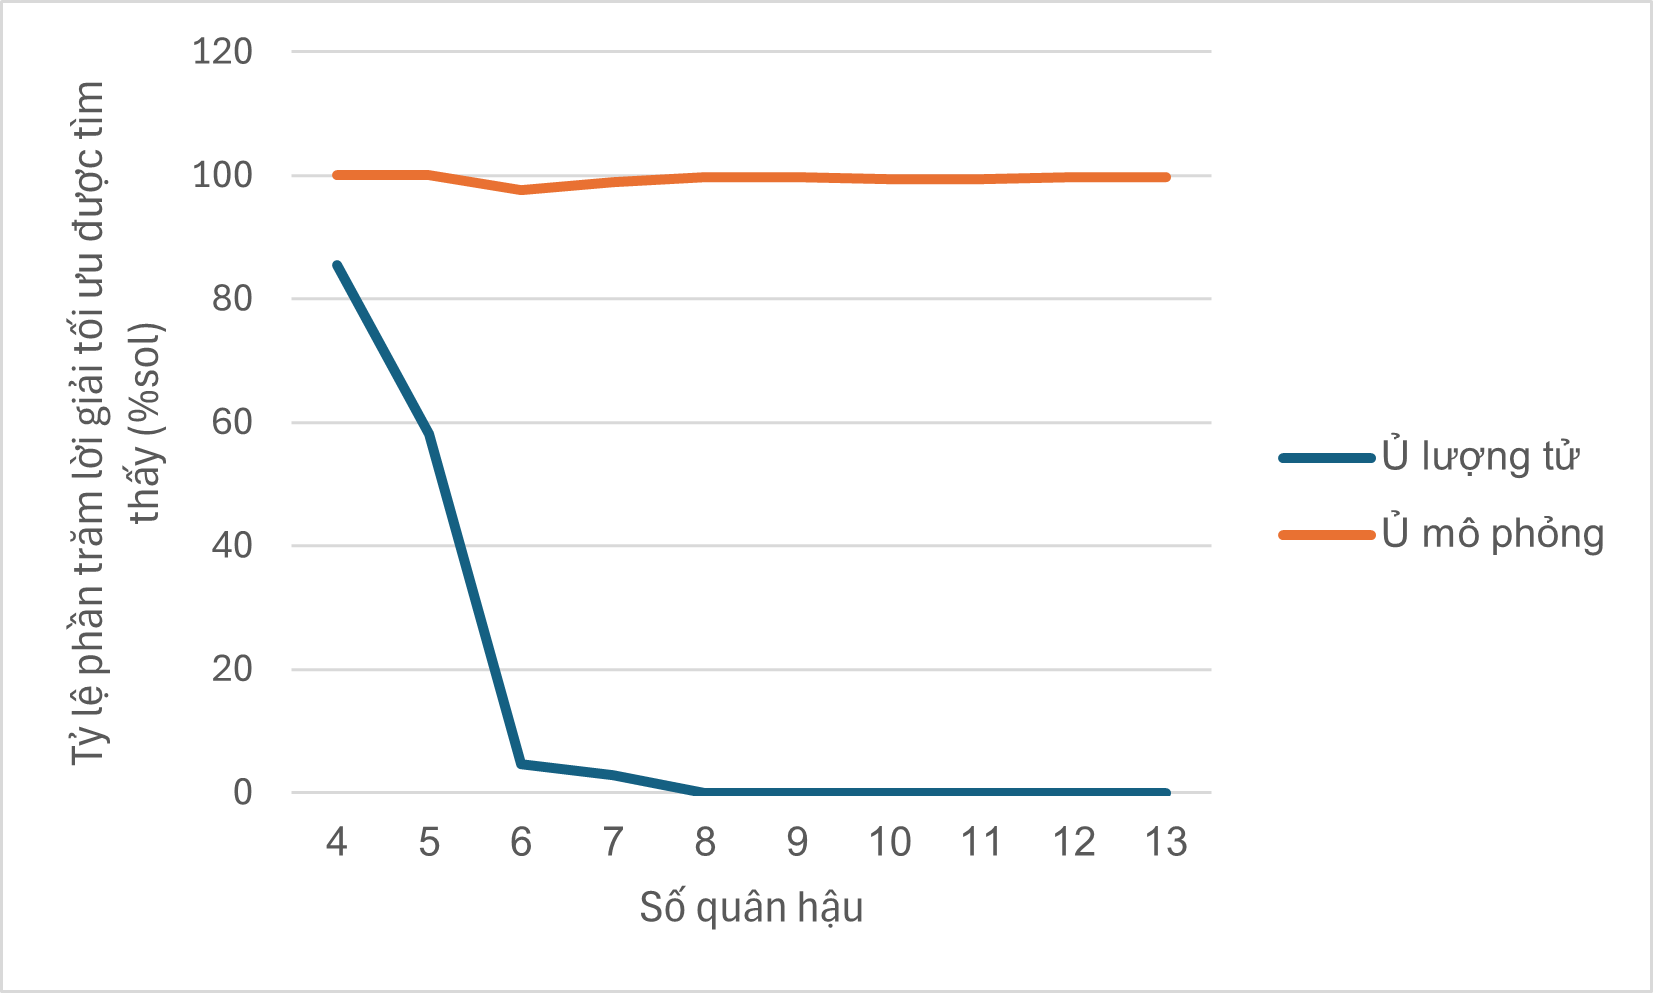
\includegraphics[width=0.7\textwidth]{images/SA_QA/sol.png}
		\caption{Biểu đồ tỷ lệ phần trăm lời giải tối ưu ($\%sol$)  của ủ lượng tử và ủ mô phỏng theo số quân hậu}
		\label{fig:SA_QA/sol}
	\end{figure}
	
	
	\begin{table}[H]
		\centering
		\begin{tabular}{|c|c|c|c|c|}
			\hline
			N & 4 & 5 & 6 & 7 \\
			\hline
			Ủ lượng tử & 0.1418 & 0.2358 & 4.1169 & 6.9181 \\
			\hline
			Ủ mô phỏng & 0.2284 & 0.3914 & 0.5899 & 0.8192 \\
			\hline
		\end{tabular}
		
		
		\caption{Bảng thời gian trung bình tìm ra một lời giải (ms)  của ủ lượng tử và ủ mô phỏng theo số quân hậu}
		\label{tab:SA_QA/TTS}
	\end{table}
	\begin{figure}[H]
		\centering
		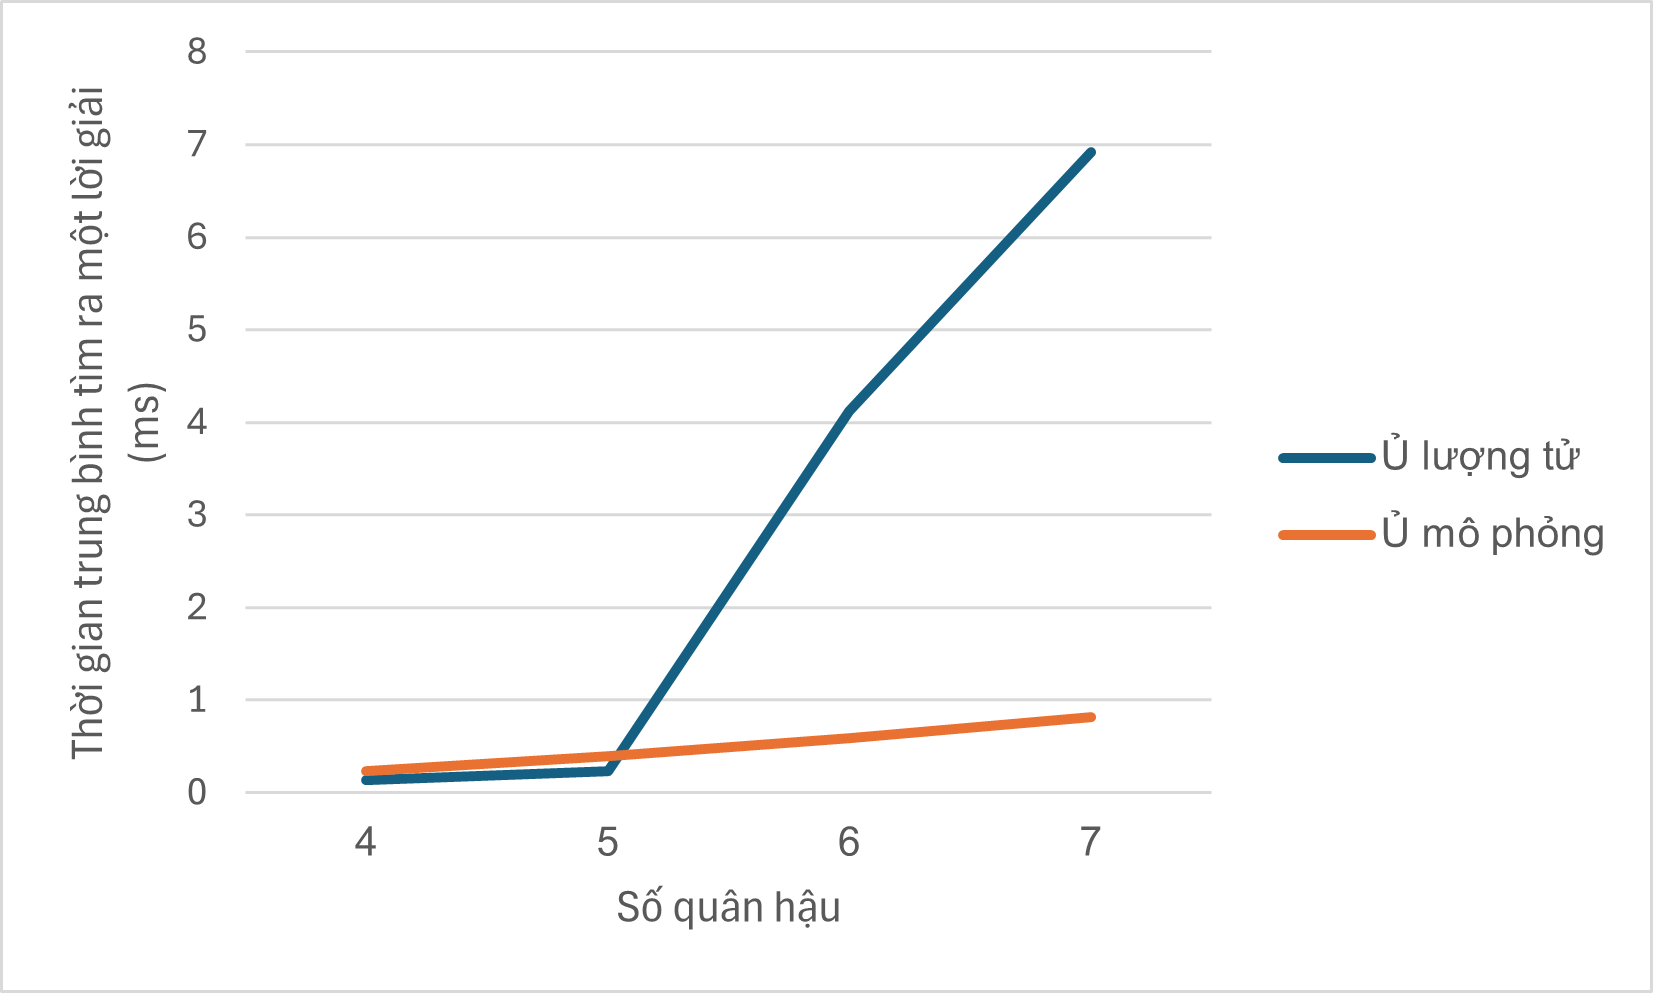
\includegraphics[width=0.7\textwidth]{images/SA_QA/TTS.png}
		\caption{Biểu đồ thời gian trung bình tìm ra một lời giải (ms)  của ủ lượng tử và ủ mô phỏng theo số quân hậu}
		\label{fig:SA_QA/TTS}
	\end{figure}
	
Như biểu diễn trong hình~\ref{fig:SA_QA/sol},~\ref{fig:SA_QA/TTS}, ủ lượng tử trong bài toán xếp hậu thực sự kém cạnh so với ủ mô phỏng cả về tỷ lệ lời giải tối ưu tìm thấy và thời gian tìm ra lời giải.
	

% Tìm hiểu thêm về các biến thể ví dụ như đã có một vài ô quân hậu được đặt trước

\chapter{Kết luận}
Chúng ta đã so sánh bài toán xếp hậu với các phương pháp cổ điển về mặt thời gian chạy. Việc tìm ra lời giải chính xác cho các bài toán tối ưu hóa lớn, phức tạp bằng các phương pháp cổ điển về cơ bản là một ngõ cụt tính toán. Không gian lời giải cho một bài toán tối ưu hóa lớn nhanh chóng vượt quá tầm kiểm soát và việc tìm kiếm trong tất cả các lời giải khả thi trở nên khó khăn.

Công thức đề xuất của chúng ta, công thức cộng dồn, tuy chưa đem đến kết quả đáng mong đợi nhưng về khía cạnh tối ưu hóa số lượng liên kết giữa các biến và chỉ yêu cầu lời giải gần đúng vẫn có thể coi là chấp nhận được.

Chúng ta cũng đã thử nghiệm và so sánh bộ lấy mẫu D-Wave với ủ mô phỏng và nhận thấy rằng thời gian chạy của nó trong bài toán xếp hậu được đánh giá không tốt. Xếp hậu là một bài toán dẫn xuất từ bài toán bao phủ chính xác, tuy nhiên ràng buộc của nó quá dày, tương tác hạt lượng tử nhiều, đặc biệt cấu trúc hạt lượng tử thưa như Pegasus sẽ yêu cầu sử dụng nhiều hạt lượng tử đã dẫn đến kết quả ủ lượng tử tệ hơn ủ mô phỏng. Hy vọng rằng cải tiến phần cứng có thể thay đổi cũng như cải thiện, khắc phục hạn chế này.

Độ phức tạp về thời gian có tác động lớn đối với quá trình ủ mô phỏng và nó không phải là hằng số. Ngược lại, quá trình ủ lượng tử thực sự có độ phức tạp về thời gian không đổi, là một điểm sáng đầy hứa hẹn.

Ủ mô phỏng là xác suất; về nguyên tắc, chúng ta có thể quyết định sự cân bằng giữa tốc độ và độ chính xác.
Trong tương lai, nếu không gian bài toán có các đặc điểm đã biết ví dụ như cho trước một vài quân hậu thì chúng ta có thể đưa ra các giả định đơn giản hóa có thể được khai thác tốt hơn. Nếu không gian bài toán của chúng ta hoàn toàn chưa được khám phá, thì tính chính xác của lời giải sẽ phụ thuộc vào tính ngẫu nhiên của không gian bài toán, thời gian chờ đợi và may mắn. Tùy theo yêu cầu cho bài toán khác nhau, việc ủ mô phỏng có thể đã đủ tốt, có khi là vượt trội.




\onecolumn

\newpage
%\chapter{Tham khảo} 


\begin{thebibliography}{}

    \bibitem{Quantum tunneling}
    \textit{Quantum tunneling in zener diodes},
    \url{https://physics.stackexchange.com/questions/466615/quantum-tunneling-in-zener-diodes}, (2019)

    \bibitem{A survey of known results and research areas for}
    J. Bell and B. Stevens, “A survey of known results and research areas for,” \textit{Discrete Mathematics}, vol. 309, no. 1, pp. 1–31, 2009.
    
      \bibitem{The computer as a physical system}
    Benioff, P., 1980. The computer as a physical system: A microscopic quantum mechanical Hamiltonian model of computers as represented by Turing machines. \textit{Journal of statistical physics}, 22, pp.563-591.

    \bibitem{Simulating physics with computers}
    Feynman, R.P., 2018. Simulating physics with computers. In \textit{Feynman and computation} (pp. 133-153). CRC Press.

    \bibitem{Quantum computational networks}

    Deutsch, D.E., 1989. Quantum computational networks. \textit{Proceedings of the royal society of London. A. mathematical and physical sciences}, 425(1868), pp.73-90.

    \bibitem{A Fast Quantum Mechanical Algorithm for Database Search}
    Grover, L.K., 1996, July. A fast quantum mechanical algorithm for database search. In \textit{Proceedings of the twenty-eighth annual ACM symposium on Theory of computing} (pp. 212-219).

    \bibitem{An approximate Fourier transform useful in quantum factoring}
    Coppersmith, D., 2002. An approximate Fourier transform useful in quantum factoring. \textit{arXiv preprint quant-ph/0201067.}

    \bibitem{Adiabatic quantum computation}
    Albash, T. and Lidar, D.A., 2018. Adiabatic quantum computation. \textit{Reviews of Modern Physics, 90(1)}, p.015002.

    \bibitem{Evidence for quantum annealing with more than one hundred qubits}
    Sergio Boixo, Troels F Rønnow, Sergei V Isakov, Zhihui Wang, David Wecker, Daniel A Lidar, John M Martinis, and Matthias Troyer. Evidence for quantum annealing with more than one hundred qubits. \textit{Nature Physics}, 10(3):218, 2014. DOI: 10.1038/nphys2900.

    \bibitem{A quantum annealin architecture with all-to-all connectivity from local interactions}
    Wolfgang Lechner, Philipp Hauke, and Peter Zoller. A quantum annealin architecture with all-to-all connectivity from local interactions. \textit{Science Advances}, 1(9), 2015. DOI: 10.1126/sciadv.1500838.

    \bibitem{Minor-embedding in adiabatic quantum computation: I. the parameter setting problem}
    Vicky Choi. Minor-embedding in adiabatic quantum computation: I. the parameter setting problem. \textit{Quantum Information Processing}, 7(5):193–209, 2008. DOI: 10.1007/s11128-008-0082-9.
  
    \bibitem{Ising formulations}
    Lucas, A., 2014. 
    \textit{Ising formulations of many NP problems. Frontiers in physics}, 2, p.74887.
  
    \bibitem{Proposal of eight queens problem}
    F. W. M. Bezzel, “Proposal of eight queens problem,” \textit{Berliner Schachzeitung}, vol. 3, p. 363, 1848.
	
    \bibitem{Topologies}
    \textit{D-Wave QPU Architecture: Topologies},
    \url{https://docs.dwavesys.com/docs/latest/c_gs_4.html}
    
    \bibitem{dynamic programming solution}
    Rivin, I. and Zabih, R., 1992. "A dynamic programming solution to the n-queens problem". 
    \textit{Information Processing Letters}, 41(5), pp.253-256.
 
    \bibitem{N Queens Dwave}
    \textit{N Queens}, \url{https://github.com/dwave-examples/n-queens} (2023).
 
    \bibitem{Problem Formulation Guide}
    \textit{Problem Formulation Guide}, \url{https://www.dwavesys.com/media/bu0lh5ee/problem-formulation-guide-2022-01-10.pdf}, (2022)
   
    \bibitem{Performance Update}
    Catherine McGeoch and Pau Farré, 
    \textit{The Advantage System: Performance Update}, (2021).
   
 
\end{thebibliography}

\end{document}